%% LyX 1.6.9 created this file.  For more info, see http://www.lyx.org/.
%% Do not edit unless you really know what you are doing.
\documentclass[oneside,english]{amsart}
%\documentclass[oneside,english]{article}\usepackage[T1]{fontenc}
\usepackage[utf8]{inputenc}
\usepackage{amsmath,amssymb,graphicx}
\usepackage{amsthm}
\usepackage{graphicx}
\usepackage{siunitx}
\usepackage{tikz}
%\usepackage{subfigure}
%\usepackage{epsfig}
%\usepackage{color}
%%%%%%%%%%%%%%%%%%%%%%%%%%%%%%%%%%%%%%%%%%%%%%%%
\graphicspath{{./Images/}}
%usepackage[dvips]{color}
%%%%%%%%%%%%%%%%%%%%%%%%%%%%%%%%%%%%%%%%%%%%%%%%%%%%%
\usepackage[left=2.5cm,right=2.5cm,top=3cm,bottom=3cm]{geometry}
%%%%%%%%%%%%%%%%%%%%%%%%%%%%%%%%%%%%%%%%%%%%%%%%%%%
%\newcommand{\cal}{\mathcal}
\newcommand{\beq}{\begin{equation}}
\newcommand{\eeq}{\end{equation}}
%%%%%%%%%%%%%%%%%%%%%%%%%%%%%%%%%%%%%%%%%%%%%%%%%%%%%
\def\sinc{\mathop{\rm sinc}\nolimits}  
\def\cal{\mathop{\rm cal}\nolimits}  
\def\cal{\mathop{\rm cal}\nolimits}  
\def\CFL{\mathop{\rm CFL}\nolimits}  
\def\VDM{\mathop{\rm VDM}\nolimits}  
\def\RK4{\mathop{\rm RK4}\nolimits}  
\def\ex{\mathop{\rm ex}\nolimits}  
\def\atan{\mathop{\rm atan}\nolimits}  
\def\sech{\mathop{\rm sech}\nolimits}  
\def\tanh{\mathop{\rm tanh}\nolimits}  
\def\div{\mathop{\rm div}\nolimits}  
\def\vort{\mathop{\rm curl}\nolimits}  
\def\vorth{\mathop{\rm curl}\nolimits}  
\def\days{\mathop{\rm days}\nolimits}  
\def\Re{\mathop{\rm Re}\nolimits}  
\def\Sp{\mathop{\rm Sp}\nolimits}  
\newcommand{\bgrad}{\mbox{\boldmath$\nabla$}}
\newcommand{\bnabla}{\mbox{\boldmath$\nabla$}}
\newcommand{\bA}{\mbox{\boldmath$A$}}
\newcommand{\bF}{\mbox{\boldmath$F$}}
\newcommand{\bP}{\mbox{\boldmath$P$}}
\newcommand{\bJ}{\mbox{\boldmath$J$}}
\newcommand{\bM}{\mbox{\boldmath$M$}}
\newcommand{\bg}{\mbox{\boldmath$g$}}
\newcommand{\bq}{\mbox{\boldmath$q$}}
\newcommand{\bx}{\mbox{\boldmath$x$}}
\newcommand{\ba}{\mbox{\boldmath$a$}}
\newcommand{\bb}{\mbox{\boldmath$b$}}
\newcommand{\bc}{\mbox{\boldmath$c$}}
\newcommand{\be}{\mbox{\boldmath$e$}}
\newcommand{\bm}{\mbox{\boldmath$m$}}
\newcommand{\bn}{\mbox{\boldmath$n$}}
\newcommand{\bu}{\mbox{\boldmath$u$}}
\newcommand{\bv}{\mbox{\boldmath$v$}}
\newcommand{\bvv}{\mathbf{v}}
\newcommand{\bs}{\mbox{\boldmath$s$}}
\newcommand{\bi}{\mbox{\boldmath$i$}}
\newcommand{\bj}{\mbox{\boldmath$j$}}
%\newcommand{\bJ}{\mbox{\boldmath$J$}}
\newcommand{\bk}{\mbox{\boldmath$k$}}
\newcommand{\bvarphi}{\mbox{\boldmath$\varphi$}}
\newcommand{\bomega}{\mbox{\boldmath$\omega$}}
\newcommand{\bpsi}{\mbox{\boldmath$\psi$}}
%%%%%%%%%%%%%%%%%%%%%%%%%%%%%%%%%%%%%%%%%%%
    \newcommand{\cJ}{\mbox{\mathcal{J}}}
    \newcommand{\fu}{\mathfrak{u}}
    \newcommand{\ftau}{\mathfrak{\tau}}
    \newcommand{\fv}{\mathfrak{v}}
    \newcommand{\fw}{\mathfrak{w}}
    \newcommand{\fz}{\mathfrak{z}}
    \newcommand{\fe}{\mathfrak{e}}
    \newcommand{\fr}{\mathfrak{r}}
    \newcommand{\fg}{\mathfrak{g}}
    \newcommand{\fq}{\mathfrak{q}}
%%%%%%%%%%%%%%%%%%%%%%%%%%%%%%%%%%%%%%%%%%%%%
% ** PERSONAL NEWTHEOREMS
\newtheorem{thm}{Theorem}[section]
\theoremstyle{definition}
\newtheorem{defi}[thm]{Definition}
\newtheorem{prop}[thm]{Proposition}
\newtheorem{coro}[thm]{Corollary}
\theoremstyle{remark}
\newtheorem{remark}[thm]{Remark}

\def\gint{\displaystyle\int}
%\def\vort{\text{vort}}
%\def\vort{\mathop{\rm curl \nolimits}  
%\newcommand{\vort}{\mbox{$\curl_\bn$}}
%\newcommand{\vorth}{\mbox{$\curl_{h,\bn}$}}

%\def\vort{\t}
\usepackage[ruled]{algorithm}
\usepackage{algpseudocode}
\alglanguage{pseudocode}


\makeatother

\usepackage{babel}

\begin{document}

\title{Numerical simulation of propagation problems on the sphere using a compact scheme}

\begin{abstract}
In this paper we consider a compact scheme 
on the sphere to approximate 
transport problems,
\cite{Croisille-10, Croisille-12}. This scheme uses 
a a crucial way the Cubed Sphere grid.
The scheme is fully centered
and used a symmetric filter to eliminate high frequency
oscillating modes. 
Numerical results on a broad series of numerical test cases
in climatology are presented, including
linear convection problems, the linearized shallow water 
and the non linear shallow water equations. 
The results demonstrate the
interest of the present approach 
in a variety of situations arising in numerical climatology.
\end{abstract}

\author{M. Brachet and J.-P. Croisille\dag\ddag}
\address{\dag Universit\'e de Lorraine, D\'epartement de Math\'ematiques, F-57045 Metz, France\\
\ddag C.N.R.S., Institut Elie Cartan de Lorraine, UMR 7502, F-57045 Metz, France}
\email{matthieu.brachet@univ-lorraine.fr, jean-pierre.croisille@univ-lorraine.fr}
\date{January, 31 2018}
\maketitle

{\sl Keywords: Cubed-Sphere grid - Compact finite difference scheme - 
Hermitian derivative - Vortex propagation}

%% **********************************************************************************************************************************************
\section{Introduction}
\label{sec:1}
In this paper we consider propagation equations on the sphere in 
climatology for the atmosphere or the ocean.
These equations are related 
to the two dimensional spherical Shallow Water equations (SWE) and
its linearizwd versions.
The SWE model represents the reference hyperbolic system
to be solved in spherical geometry. 
A second problem (LSWE) consists of the linearized SWE 
at an atmosphere at rest. This problem represents
the basic waves model on the sphere.
It is of fundamental importance 
in climatology and oceanography. On this topic, 
refer to the recent monograph \cite{Paldor}.

The SWE and LSWE systems are the source of many efforts
to adapt conservative methods  
originating from numerical gas dynamics.
This is the case of the finite volume
method \cite{Chen-Xiao, Ullrich-Jablonowski-vanLeer}.
or the Discontinuous Galerkin methods \cite{Bao-Nair-Tufo}.

In this paper, we address 
the particular finite difference scheme 
introduced in \cite{Croisille-10,Croisille-12}.
This scheme is compact 

Among the classical methods for fluid flows, the 
scheme is strongly related to 
compact schemes used in computational aeroacoustic
\cite{Lele, Visbal-Gaitonde, 
Tam-Webb, Bogey-Bailly} and in turbulence \cite{Kim-Moin}.
The originality lies in the fact
that it operates on the Cubed Sphere grid at the global level. 
Our approach can be traced back to early works
in approximation and interpolation theory, \cite{Collatz}.
In the particular field of numerical climatology, 
our approach is related to \cite{Arakawa} and more recently
to the compact scheme presented in \cite{Ghader-Nordstrom}.
Our scheme is fully centered and no upwinding
is introduced. A simple high frequency filtering
is added for stabilization purpose. 
In addition, only one value per gridpoint is used.

Three convective models are considered in the sequel:
\begin{itemize}
\item 
The spherical advection equation is: 
\begin{equation}
\label{eq:adv}
\dfrac{\partial h}{\partial t}  (t,\mathbf{x})+ \mathbf{c}(t,\mathbf{x}) 
\cdot \nabla_T h(t,\mathbf{x})=0
\end{equation}
The velocity
$\mathbf{c}(t,\mathbf{x}) \in \mathbb{T}\mathbb{S}^2$ 
is a prescribed tangential vector field.
This linear problem is essential in climatology. The scalar $h(t,x)$ typically 
represents the density of a pollutant convected by the wind with 
velocity $\bc$. 
The numerical solution is compared to 
the analytical solution. This permits 
to evaluate, not only the dissipation and the dispersion,
but also the long time behaviour of the scheme,
which is essential for assess the prediction capabilities
of the procedure. 
\item
The linearized Shallow Water model (LSWE) linearized at 
an atmosphere at rest $q_0=[H,\mathbf{v}=\mathbf{0}]$  is
\begin{equation}
\label{eq:lswe}
(LSWE) \left\{
\begin{array}{l}
\dfrac{\partial \eta}{\partial t} (t,\mathbf{x})+ H \nabla_T 
\cdot \mathbf{v}(t,\mathbf{x})=S_\eta(t,\bx)\\
\dfrac{\partial \mathbf{v} }{\partial t} (t,\mathbf{x})+ 
g \nabla_T \eta(t,\mathbf{x}) + f(\mathbf{x}) \mathbf{k}(\mathbf{x}) \times
\mathbf{v}(t,\mathbf{x})=S_{\bv}(t,\bx)\\
\end{array}
\right.
\end{equation}
This system is the basic model for wave problems 
on the sphere since Laplace. It represents the small perturbations
of the atmosphere height $\eta$ and velocity $\bv$.
The source terms $S_\eta$ and $S_{\bv}$ stand for forcing functions.
The vector function $\bx f(\bx) \bk \times \bv$ represents the Coriolis force.
This wave problem still offers many mathematical open questions \cite{Paldor}.
Acurate numerical simulations are important to get insight in this problem.
\item The full SWE system is nonlinear. It is expressed 
in vector form as:
\begin{equation}
\label{eq:swe}
(SWE) \left\lbrace
\begin{array}{l}
\dfrac{\partial h^{\star}}{\partial t} (t,\mathbf{x}) + \nabla_T \cdot \left( h^{\star}(t,\mathbf{x}) \mathbf{v}(t,\mathbf{x}) \right) =  0 \\
\dfrac{\partial \mathbf{v}}{\partial t}  (t,\mathbf{x}) + \nabla_T \left( \dfrac{1}{2} |\mathbf{v}(t,\mathbf{x})|^2 
+ g h(t,\mathbf{x}) \right) + \left( f(\mathbf{x}) + \zeta(t,\mathbf{x}) \right) \mathbf{n}(\mathbf{x}) \times \mathbf{v}(t,\mathbf{x}) =  \mathbf{0} 
\end{array}
\right.
\end{equation}
where $\zeta = \left( \nabla_T \times \mathbf{v} \right) \cdot \mathbf{n}$ 
is the {\it relative vorticity} and 
$h^{\star} = h - h_s$ with $h_s$ the bottom topography function.
\end{itemize}
For these three models, 
we show that our centered scheme compares 
favourably to traditional conservative upwind methods,
such as the finite volume method \cite{Ullrich-Jablonowski-vanLeer}
or the Discoutinuous Galerkin method \cite{Nair-Choi-Tufo}.

The vector form (\ref{eq:swe}) is nonconservative. 
It is adopted here, mainly
due to its simplicity,
compared to the conservative form, \cite{Bao-Nair-Tufo}.
Since our scheme is a priori not conservative,
we need to carefully evaluate how evolve the conserved quantities.
These conserved quantities are not only 
primary conserved quantities such as the mass
and the energy, but also potential enstrophy or the 
angular momentum.
However other quantities,
which are theoretically conserved by SWE,
such as the potential enstrophy 
can suffer excessive dissipation
for large time, when upwind methods are used.
This is why we analyze the conservation
properties of our scheme
as a whole, with particular attention to
the conservation for large time. 

The outline of the paper is as follows.
In Section \ref{sec:2}, we recall the essential of 
our approach along the lines 
of \cite{Croisille-10, Croisille-12}. In Sec \ref{sec:num}, we present 
numerical results on a series of test cases
involving (\ref{eq:adv}), (\ref{eq:lswe}) and (\ref{eq:swe}). 
Finally, in Section \ref{sec:annexes}
some analysis of the basic compact scheme is carried out on the 
model of the linear advection equation in a periodic setting.
This includes
a convergence analysis of the standard 4th order compact scheme 
as well as the stablity matrix analysis of the fully 
discrete scheme, including filtering.
%%%%%%%%%%%%%%%%%%%%%%%%%%%%%%%%%%%%%%%%%%%%%%%%%%%%%%%%%%%%%%%%%
\section{Numerical scheme using central compact differencing 
on the Cubed Sphere}
\label{sec:2}
In this section, we review the basic of our compact scheme.
This scheme uses a particular property of the Cubed Sphere,
the fact that coordinate lines are great circles sections.
These great circles are then used
as a support 
for compact finite difference scheme.
Here we use the standard
fourth order Hermitian scheme.
This approach allows to evaluate 
accurate versions of the gradient, divergence and curl
on the sphere.
%% ********************************************************
\subsection{The Cubed-Sphere}
\label{sec:CS}
The Cubed Sphere \cite{Sadourny} is a spherical grid widely used
in numerical climatology .
A modern presentation was given in
\cite{Ronchi-Iacono-Paolucci}.
It is composed of six panels 
labeled with the index 
$k=(I), (II), (II), (IV), (V)$ and $(VI)$. Each panel 
matches the face of a cube and
supports a Cartesian grid of size $(N+1)\times (N+1)$.
The integer $N$ represents the spatial resolution.
Each panel is equipped with a 
coordinate system $(\xi,\eta)$.
The coordinate lines consist of two angles
measured along the two "equatorial" great circles 
intersecting at the center.
The Cubed Sphere is represented on Fig. \ref{fig:1}
and a typical panel is shown
on Fig. \ref{fig:2}.
%%%%%%%%%%%%%%%%%%%%%%%%%%%%%%%%%%%%%%%%%%%%%%%%%%%%%%%%%%%%%%%%
\begin{figure}
\includegraphics[scale=0.4]{Images/fig6.jpg}
\caption{
The Cubed Sphere with resolution parameter $N=16$.
The number of gridpoints is $6 N^2+2$, ($1538$ in this case).
The four panels $(I)$, $(II)$, $(III)$ and $(IV)$ are located
around the equatorial plane $z=0$. 
The indices of the north and south panels are $(V)$ 
and $(VI)$ respectively. 
}
\label{fig:1}
\end{figure}
%%%%%%%%%%%%%%%%%%%%%%%%%%%%%%%%%%%%%%%%%%%%%%%%%%%%%%
\begin{figure}
   \def\svgwidth{0.3 \textwidth}
\input{drawing13.pdf_tex}
\caption{
Frontal view of a panel. 
The points of a typical panel of the Cubed-Sphere are 
classified in three categories:
(i) $(N-1)^2$ circles correspond to the {\sl internal} points; 
(ii) $4 (N-1)^2$ squares 
correspond to the {\sl edge} points ;
(iii) $4$ pentagons correspond to the {\sl corner} points}
\label{fig:2}
\end{figure}
%%%%%%%%%%%%%%%%%%%%%%%%%%%%%%%%%%%%%%%%%%%%%%%%%%%%%%
The points on panel $k$ are denoted 
$\mathbf{s}_{i,j}^{k}$
The integer $i$ (resp. $j$) 
denotes the index in the $\xi$ direction (resp. $\eta$) direction.
Our finite difference scheme uses discrete unknowns
located at the points $\mathbf{s}^{k}_{i,j}$.
%%%%%%%%%%%%%%%%%%%%%%%%%%%%%%%%%%%%%%%%%%%%%%%%%%%
\subsection{Great circles on the Cubed Sphere}
\label{sec:der_cs}
The spatial approximation used in this papeer is based on the standard 
Hermitian derivative. We refer to
\cite{Collatz, Lele, Gustafsson-4, BenArtzi-Croisille-Fishelov}. 
Suppose given $u_j$ a set of data at points $x_j =j \Delta x$.
The approximate derivatives $\delta_x^H u_j$ are 
obtained by solving the tridiagonal system
\beq
\label{eq:812.45}
\frac{1}{6}\delta^H_x u_{j-1}+
\frac{2}{3}\delta^H_x u_j+
\frac{1}{6}\delta^H_x u_{j+1}
=\frac{u_{j+1}-u_{j-1}}{2 \Delta x}.
\eeq
The approximate derivative $\delta^H u_j$
is fourth order accurate with truncation error
\beq
\label{eq:18:312}
\delta_x^H u_{j}-u^\prime(x_j)=-\frac{1}{180}h^4 u^{(5)}(x_j)+ O(h^6)
\eeq
Here, the main idea consists
in using (\ref{eq:812.45}) along a particular set of great circles
on the Cubed Sphere. This set will be defined hereafter.
This permits
to approximate with high accuracy 
the spherical gradient, the divergence and the 
vorticity on the sphere.
This is suggested by the fact that
coordinate lines are great circle sections.
%Two typical such great circles are represented
%in Fig. \ref{fig:patron cs}.
%%%%%%%%%%%%%%%%%%%%%%%%%%%%%%%%%%%%%%%%%%%%%%%%%%%%%
\begin{figure}
\begin{center}
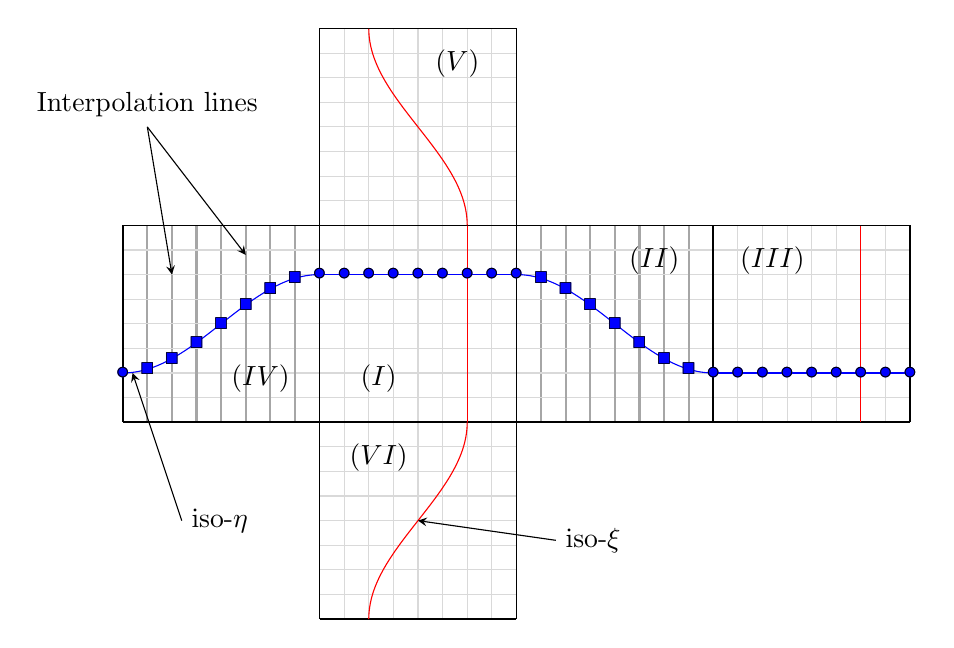
\begin{tikzpicture}[scale=2.5]
	\foreach \x in {1,...,7}
		{ \draw [color=gray!70, line width=0.8pt] (0.125*\x,1) -- (0.125*\x,2) ;
		\draw [color=gray!30] (0,1+0.125*\x) -- (1,1+0.125*\x) ;
		\draw [color=gray!30] (1+0.125*\x,1) -- (1+0.125*\x,2) ;
		\draw [color=gray!30] (1,1+0.125*\x) -- (2,1+0.125*\x) ;
		\draw [color=gray!70, line width=0.8pt] (2+0.125*\x,1) -- (2+0.125*\x,2) ;
		\draw [color=gray!30] (2,1+0.125*\x) -- (3,1+0.125*\x) ;
		\draw [color=gray!30] (3+0.125*\x,1) -- (3+0.125*\x,2) ;
		\draw [color=gray!30] (3,1+0.125*\x) -- (4,1+0.125*\x) ;
		\draw [color=gray!30] (1+0.125*\x,0) -- (1+0.125*\x,1) ;
		\draw [color=gray!30] (1,0.125*\x) -- (2,0.125*\x) ;
		\draw [color=gray!30] (1+0.125*\x,2) -- (1+0.125*\x,3) ;		
		\draw [color=gray!30] (1,2+0.125*\x) -- (2,2+0.125*\x) ;
		}
	

	\draw [line width=0.6pt] (1,3) -- (2,3) ; 
	\draw [line width=0.6pt] (0,2) -- (4,2) ; 	
	\draw [line width=0.6pt] (0,1) -- (4,1) ; 
	\draw [line width=0.6pt] (1,0) -- (2,0) ; 
	
	\draw [line width=0.6pt] (0,2) -- (0,1) ;
	\draw [line width=0.6pt] (1,3) -- (1,0) ;
	\draw [line width=0.6pt] (2,3) -- (2,0) ;
	\draw [line width=0.6pt] (3,2) -- (3,1) ;
	\draw [line width=0.6pt] (4,2) -- (4,1) ; 
	
	\draw (0.7,1.1) node[above]{$(IV)$} ; 
	\draw (1.3,1.1) node[above]{$(I)$} ; 
	\draw (2.7,1.7) node[above]{$(II)$} ;
	\draw (3.3,1.7) node[above]{$(III)$} ;  
	\draw (1.7,2.7) node[above]{$(V)$} ;  
	\draw (1.3,0.7) node[above]{$(VI)$} ; 
	
	\draw [samples=100,domain=0:1,color=blue] plot({\x},{1.5-(2*0.125)*cos(180*\x)});
	\draw [samples=100,domain=1:2,color=blue] plot({\x},{1.5+2*0.125});
	\draw [samples=100,domain=1:2,color=blue] plot({\x+1},{1.5-2*0.125*cos(180*\x)});
	\draw [samples=100,domain=3:4,color=blue] plot({\x},{1.5-2*0.125});
	\draw [>=stealth, <-] (0.05,1.25) -- (0.3,0.5) ;
	\draw  (0.3,0.5) node[right] {iso-$\eta$} ;
	
	\draw [samples=100,domain=0:1,color=red] plot({1.5-2*0.125*cos(180*\x)},{\x});
	\draw [samples=100,domain=1:2,color=red] plot({1.5+2*0.125},{\x});
	\draw [samples=100,domain=1:2,color=red] plot({1.5-2*0.125*cos(180*\x)},{\x+1});
	\draw [samples=100,domain=1:2,color=red] plot({4-+2*0.125},{\x});
	\draw [>=stealth, <-] (1.5,0.5) -- (2.2,0.4) ;
	\draw  (2.2,0.4) node[right] {iso-$\xi$} ;
	
	\draw  (0,1+2*0.125) node[color=blue] {$\bullet$} ;
	\draw (0,1+2*0.125) node {$\circ$} ;
	
	\foreach \k in {0,...,8}
		{\draw  (1+0.125*\k,1.5+2*0.125) node[color=blue] {$\bullet$} ;
	   	\draw (1+0.125*\k,1.5+2*0.125) node {$\circ$} ;
	   	\draw  (3+0.125*\k,1+2*0.125) node[color=blue] {$\bullet$} ;
	   	\draw (3+0.125*\k,1+2*0.125) node {$\circ$} ;
	   	}
	   	
	\foreach \x in {1,...,7}
		{\draw  ({0.125*\x},{1.5-2*0.125*cos(180*0.125*\x)}) node[color=blue] {\begin{tiny}$\blacksquare$\end{tiny}} ;
	   	\draw ({0.125*\x},{1.5-2*0.125*cos(180*0.125*\x)}) node {\begin{tiny}$\square$\end{tiny}} ;
	   	\draw  ({2+0.125*\x},{1.5-2*0.125*cos(180*0.125*\x+180)}) node[color=blue] {\begin{tiny}$\blacksquare$\end{tiny}} ;
	   	\draw  ({2+0.125*\x},{1.5-2*0.125*cos(180*0.125*\x+180)}) node {\begin{tiny}$\square$\end{tiny}} ;
	   	}
	   	
	\draw [>=stealth, <-] (0.25,1.75) -- (0.125,2.5) ;
	\draw [>=stealth, <-] (0.625,1.85) -- (0.125,2.5) ;
	\draw  (0.125,2.5) node[above] {Interpolation lines} ;
\end{tikzpicture}
\caption{Two typical great circles associated to
coordinate lines along the Cubed Sphere.
Periodic compact differencing \ref{eq:812.45} is carried out along each circle,
giving one-dimensional approximate derivatives.
Points marked with circles correspond to 
gridpoints where values are available. In the contrary,
values must be interpolated at points marked with squares.}
\label{fig:patron cs}
\end{center}
\end{figure}
%%%%%%%%%%%%%%%%%%%%%%%%%%%%%%%%%%%%%%%%%%%%%%%%%%%%%%%%%%%%%%%%%%%%%%%
\begin{figure}[htbp]
\begin{center}
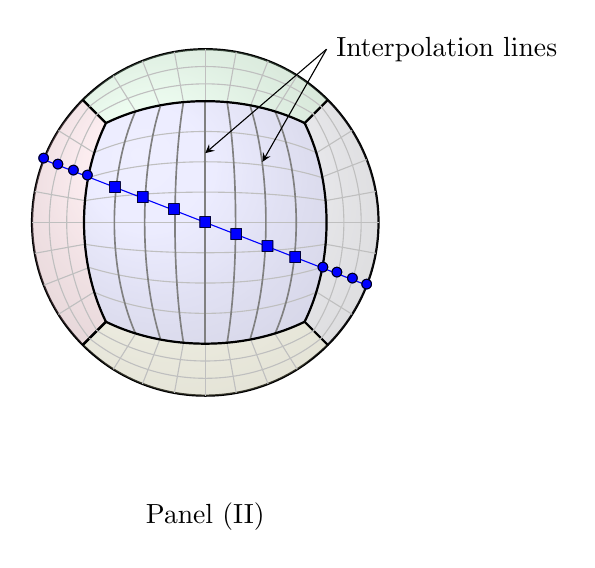
\begin{tikzpicture}[scale=2.2]
	\draw [line width=0.8pt] (0,0) circle (1cm);
    \shade[ball color=blue!10!white,opacity=0.20] (0,0) circle (1cm);	
	
	\filldraw[draw=black,fill=blue!30!white,opacity=0.20]
	plot [smooth,domain=-35:35] ({0.7*cos(\x)},{sin(\x)})
	-- plot [smooth,domain=55:125] ({cos(\x)},{0.7*sin(\x)})
	-- plot [smooth,domain=150:215] ({0.7*cos(\x)},{sin(\x)})
	-- plot [smooth,domain=240:300] ({cos(\x)},{0.7*sin(\x)})
	-- cycle;	
	\draw [samples=100,domain=48:132, color=gray!50] plot({cos(\x)},{0.35*sin(\x)});
	\draw [samples=100,domain=48:132, color=gray!50] plot({cos(\x)},{-.35*sin(\x)});
	\draw [samples=100,domain=46:134, color=gray!50] plot({cos(\x)},{0.175*sin(\x)});
	\draw [samples=100,domain=46:134, color=gray!50] plot({cos(\x)},{-.175*sin(\x)});
	\draw [samples=100,domain=50:130, color=gray!50] plot({cos(\x)},{0.525*sin(\x)});
	\draw [samples=100,domain=50:130, color=gray!50] plot({cos(\x)},{-.525*sin(\x)});
	\draw [samples=100,domain=45:135, color=gray!50] plot({cos(\x)},{0*sin(\x)});

	\draw [rotate=90, samples=100,domain=48:132, color=gray, line width=0.6pt] plot({cos(\x)},{0.35*sin(\x)});
	\draw [rotate=90, samples=100,domain=48:132, color=gray, line width=0.6pt] plot({cos(\x)},{-.35*sin(\x)});
	\draw [rotate=90, samples=100,domain=46:134, color=gray, line width=0.6pt] plot({cos(\x)},{0.175*sin(\x)});
	\draw [rotate=90, samples=100,domain=46:134, color=gray, line width=0.6pt] plot({cos(\x)},{-.175*sin(\x)});
	\draw [rotate=90, samples=100,domain=50:130, color=gray, line width=0.6pt] plot({cos(\x)},{0.525*sin(\x)});
	\draw [rotate=90, samples=100,domain=50:130, color=gray, line width=0.6pt] plot({cos(\x)},{-.525*sin(\x)});
	\draw [rotate=90, samples=100,domain=45:135, color=gray, line width=0.6pt] plot({cos(\x)},{0*sin(\x)});

	\filldraw[draw=black,fill=red!30!white,opacity=0.20]
	plot [smooth,domain=145:215] ({.7*cos(\x)},{sin(\x)})
	-- plot [smooth] (-.573,-.573) -- (-.707,-.707)
	-- plot [smooth,domain=215:145] ({cos(\x)},{sin(\x)})
	-- plot [smooth] (-.707,.707) -- (-.573,.573)
	-- cycle;	
	\draw [line width=0.8pt] (-.573,-.573) -- (-.707,-.707) ;
	\draw [line width=0.8pt] (-.573,.573) -- (-.707,.707) ;
	\draw [color=gray!50] (-.669,.260) -- (-.9321,.3622) ;
	\draw [color=gray!50] (-.669,-.260) -- (-.9321,-.3622) ;
	\draw [color=gray!50] (-.6946,.1259) -- (-.9840,.1783) ;
	\draw [color=gray!50] (-.6946,-.1259) -- (-.9840,-.1783) ;
	\draw [color=gray!50] (-.6427,.4022) -- (-.8477,.5305) ;
	\draw [color=gray!50] (-.6427,-.4022) -- (-.8477,-.5305) ;
	\draw [color=gray!50] (-.707,0) -- (-1,0) ;
	\draw [samples=100,domain=141:219, color=gray!50] plot({0.8*cos(\x)},{sin(\x)});
	\draw [samples=100,domain=138:222, color=gray!50] plot({0.9*cos(\x)},{sin(\x)});
	
	\filldraw[draw=black,fill=green!30!white,opacity=0.20]
	plot [smooth,domain=55:125] ({cos(\x)},{0.7*sin(\x)})
	-- plot [smooth] (-.573,.573) -- (-.707,.707)
	-- plot [smooth,domain=125:55] ({cos(\x)},{sin(\x)})
	-- plot [smooth] (.707,.707) -- (.573,.573)
	-- cycle;	
	\draw [line width=0.8pt] (-.573,.573) -- (-.707,.707) ;
	\draw [line width=0.8pt] (.707,.707) -- (.573,.573) ;
	\draw [rotate=-90,color=gray!50] (-.669,.260) -- (-.9321,.3622) ;
	\draw [rotate=-90,color=gray!50] (-.669,-.260) -- (-.9321,-.3622) ;
	\draw [rotate=-90,color=gray!50] (-.6946,.1259) -- (-.9840,.1783) ;
	\draw [rotate=-90,color=gray!50] (-.6946,-.1259) -- (-.9840,-.1783) ;
	\draw [rotate=-90,color=gray!50] (-.6427,.4022) -- (-.8477,.5305) ;
	\draw [rotate=-90,color=gray!50] (-.6427,-.4022) -- (-.8477,-.5305) ;
	\draw [rotate=-90,color=gray!50] (-.707,0) -- (-1,0) ;
	\draw [rotate=-90,samples=100,domain=141:219, color=gray!50] plot({0.8*cos(\x)},{sin(\x)});
	\draw [rotate=-90,samples=100,domain=138:222, color=gray!50] plot({0.9*cos(\x)},{sin(\x)});
	
	\filldraw[draw=black,fill=yellow!30!white,opacity=0.20]
	plot [smooth,domain=55:125] ({cos(\x)},{-.7*sin(\x)})
	-- plot [smooth] (-.573,-.573) -- (-.707,-.707)
	-- plot [smooth,domain=125:55] ({cos(\x)},{-sin(\x)})
	-- plot [smooth] (.707,-.707) -- (.573,-.573)
	-- cycle;	
	\draw [line width=0.8pt] (-.573,-.573) -- (-.707,-.707) ;
	\draw [line width=0.8pt] (.707,-.707) -- (.573,-.573) ;
	\draw [rotate=90,color=gray!50] (-.669,.260) -- (-.9321,.3622) ;
	\draw [rotate=90,color=gray!50] (-.669,-.260) -- (-.9321,-.3622) ;
	\draw [rotate=90,color=gray!50] (-.6946,.1259) -- (-.9840,.1783) ;
	\draw [rotate=90,color=gray!50] (-.6946,-.1259) -- (-.9840,-.1783) ;
	\draw [rotate=90,color=gray!50] (-.6427,.4022) -- (-.8477,.5305) ;
	\draw [rotate=90,color=gray!50] (-.6427,-.4022) -- (-.8477,-.5305) ;
	\draw [rotate=90,color=gray!50] (-.707,0) -- (-1,0) ;
	\draw [rotate=90,samples=100,domain=141:219, color=gray!50] plot({0.8*cos(\x)},{sin(\x)});
	\draw [rotate=90,samples=100,domain=138:222, color=gray!50] plot({0.9*cos(\x)},{sin(\x)});
	
	\draw [rotate=180,color=gray!50] (-.669,.260) -- (-.9321,.3622) ;
	\draw [rotate=180,color=gray!50] (-.669,-.260) -- (-.9321,-.3622) ;
	\draw [rotate=180,color=gray!50] (-.6946,.1259) -- (-.9840,.1783) ;
	\draw [rotate=180,color=gray!50] (-.6946,-.1259) -- (-.9840,-.1783) ;
	\draw [rotate=180,color=gray!50] (-.6427,.4022) -- (-.8477,.5305) ;
	\draw [rotate=180,color=gray!50] (-.6427,-.4022) -- (-.8477,-.5305) ;
	\draw [rotate=180,color=gray!50] (-.707,0) -- (-1,0) ;
	\draw [rotate=180,samples=100,domain=141:219, color=gray!50] plot({0.8*cos(\x)},{sin(\x)});
	\draw [rotate=180,samples=100,domain=138:222, color=gray!50] plot({0.9*cos(\x)},{sin(\x)});
	
	\draw [samples=100,domain=55:125, line width=0.8pt] plot({cos(\x)},{0.7*sin(\x)});
	\draw [samples=100,domain=55:125, line width=0.8pt] plot({cos(\x)},{-.7*sin(\x)});
	\draw [samples=100,domain=145:215, line width=0.8pt] plot({.7*cos(\x)},{sin(\x)}); 
	\draw [samples=100,domain=145:215, line width=0.8pt] plot({-.7*cos(\x)},{sin(\x)}); 
	
	\draw [color=blue] (-.9321,.3622) -- (.9321,-.3622) ;
	\draw  (-.9321,.3622) node[color=blue] {$\bullet$} ;
	\draw (-.9321,.3622) node {$\circ$} ;	
	\draw  (.9321,-.3622) node[color=blue] {$\bullet$} ;
	\draw (.9321,-.3622) node {$\circ$} ;
	\draw  (-.85,0.3886*.85) node[color=blue] {$\bullet$} ;
	\draw (-.85,0.3886*.85) node {$\circ$} ;	
	\draw (.85,-0.3886*.85) node[color=blue] {$\bullet$} ;
	\draw (.85,-0.3886*.85) node {$\circ$} ;	
	\draw  (-.76,0.3886*.76) node[color=blue] {$\bullet$} ;
	\draw (-.76,0.3886*.76) node {$\circ$} ;	
	\draw (.76,-0.3886*.76) node[color=blue] {$\bullet$} ;
	\draw (.76,-0.3886*.76) node {$\circ$} ;
	\draw  (-.68,0.3886*.68) node[color=blue] {$\bullet$} ;
	\draw (-.68,0.3886*.68) node {$\circ$} ;	
	\draw (.68,-0.3886*.68) node[color=blue] {$\bullet$} ;
	\draw (.68,-0.3886*.68) node {$\circ$} ;	
	\draw (-.52,0.3886*.52) node[color=blue] {\begin{tiny}$\blacksquare$ \end{tiny}} ;
	\draw (-.52,0.3886*.52) node {\begin{tiny}$\square$ \end{tiny}} ;
	\draw (.52,-0.3886*.52) node[color=blue] {\begin{tiny}$\blacksquare$ \end{tiny}} ;
	\draw (.52,-0.3886*.52) node {\begin{tiny}$\square$ \end{tiny}} ;
	\draw (-.36,0.3886*.36) node[color=blue] {\begin{tiny}$\blacksquare$ \end{tiny}} ;
	\draw (-.36,0.3886*.36) node {\begin{tiny}$\square$ \end{tiny}} ;
	\draw (.36,-0.3886*.36) node[color=blue] {\begin{tiny}$\blacksquare$ \end{tiny}} ;
	\draw (.36,-0.3886*.36) node {\begin{tiny}$\square$ \end{tiny}} ;
	\draw (-.18,0.3886*.18) node[color=blue] {\begin{tiny}$\blacksquare$ \end{tiny}} ;
	\draw (-.18,0.3886*.18) node {\begin{tiny}$\square$ \end{tiny}} ;
	\draw (.18,-0.3886*.18) node[color=blue] {\begin{tiny}$\blacksquare$ \end{tiny}} ;
	\draw (.18,-0.3886*.18) node {\begin{tiny}$\square$ \end{tiny}} ;
	\draw (0,0) node[color=blue] {\begin{tiny}$\blacksquare$ \end{tiny}} ;
	\draw (0,0) node {\begin{tiny}$\square$ \end{tiny}} ;
	
	\draw [>=stealth, <-] (.33,.35) -- (.7,1) ;
	\draw [>=stealth, <-] (0,.4) -- (.7,1) ;
	\draw  (0.7,1) node[right] {Interpolation lines} ;
	
	\draw  (0,-1.7) node {Panel (II)} ;

\end{tikzpicture}
\end{center}
\caption{The great circle of Fig. \ref{fig:patron cs}
is shown. The points marked with squares are located on panel (II).
The value assigned to each point is deduced 
by a spline interpolation along each vertical line.
This serves the purpose to evaluate accurately the
derivative along the circle according to the compact formula (\ref{}).}
\label{fig: panel II_interp}
\end{figure}  
%%%%%%%%%%%%%%%%%%%%%%%%%%%%%%%%%%%%%%%%%%%%%%%%%%%%%%%%%%%%%%%%%
Consider for example in Fig. \ref{fig:patron cs}.
the great circle crossing panels
$(I),(II),(III)$ and $(IV)$.
This circle coincides with coordinate lines in panels $(I)$ and $(III)$.
In panels $(II)$ and $((IV)$ it does not conicide with
coordinate lines.
Consider now evaluating the gradient $\nabla_T f$
of some function $f$. 
Denote $(f^\ast)^k_{i,j}$ the restriction of $f$ at the 
Cubed Sphere points.
Based on the values $(f^\ast)^k_{i,j}$ 
one can calculate Hermitian derivatives
along this circle. 
First a suitable set of points is defined on this circle.
Second values $f_p$ are assigned to these points. And third
$\delta^H_x f_{p}$ using (\ref{eq:812.45}).

Consider the sphere $\Bbb S_a$ with radius $a$.
The Cubed Sphere grid is set up on $\Bbb S_a$ with points
$\bs^k_{i,j}$. 
On each panel $k$, $(I) \leq k \leq (VI)$, the local basis 
$(\bg_\xi,\bg_\eta)$ is
is 
\beq
\label{eq:32.19}
\bg_\xi(\mathbf{x})=\frac{\partial \mathbf{x}}{\partial \xi},\;\;\;
\bg_\eta(\mathbf{x})=\frac{\partial \mathbf{x}}{\partial \eta}.
\eeq
Let $f(\bx)$ be a regular function defined on $\Bbb S_a$.
Te restriction of $f$ to the Cubed Sphere is 
called $f^\ast$ with $(f^\ast)^k_{i,j} = f(\mathbf{s}_{i,j}^k)$.

The gradient of $f(\bx)$ is expressed in terms of the dual basis 
$(\bg^\xi, \bg^\eta)$ by
\begin{equation}
\nabla_T f(\bx) = \dfrac{\partial f}{\partial \xi}(\bx) \mathbf{g}^{\xi}(\bx) 
+ \dfrac{\partial f}{\partial \eta}(\bx) \mathbf{g}^{\eta}(\bx)
\label{eq:gradient}
\end{equation}
Consider now two approximate derivative of the form
\beq
\dfrac{\partial f}{\partial \xi} \simeq \delta^H_\xi f^k_{i,j},\;\;\;
\dfrac{\partial f}{\partial \eta} \simeq \delta^H_\eta f^k_{i,j}.
\eeq
where the Hermitian derivative $\delta^H_\xi f^k_{i,j}$
and $\delta^H_\eta f^k_{i,j}$ are to be calculated along great circles.
A natural approximate gradient is 
\begin{equation}
\nabla_{T,\Delta} (f^\ast)_{i,j}^k 
=\delta^H_\xi (f^\ast)_{i,j}^k \mathbf{g}^{\xi} 
\delta^H_\eta (f^\ast)_{i,j}^k \mathbf{g}^{\eta}. 
\label{eq:gradient_app}
\end{equation}
where $\delta_\xi^H f^{k}_{i,j}$ and 
$\delta_\eta^H f^{k}_{i,j}$ are evaluated using (\ref{eq:812.45}).

The detailed computational procedure proceeds in four steps
according to Algorithm \ref{algo:4} hereafter. 
Consider in Fig. \ref{fig:patron cs} the circle 
in horizontal position. This circle corresponds to some iso-$\eta$ line $\eta=\eta_0$
in panel (I).
%%%%%%%%%%%%%%%%%%%%%%%%%%%%%%%%%%%%%%%%%%%%%%%%%%%%%%%%%%
%\begin{flushleft}
%\begin{algorithm}
%\label{algo:4}
%\noindent
%$\bullet$ {\bf Step 1:}{\sl Grid along the circle}.\\
%A grid of $4 N$ points $\bm_p$, $p=0,\dots,4N$ is defined on the circle 
%as follow:
%\begin{enumerate}
%\item The points $\bm_p = \bs^{(I)}_{p-N/2,j_0}$, $p=0, ..., N-1$. 
%These points belong to panel (I). They are gridpoints and they carry 
%values $u^{(I)}_{i,j_0}$. They are represented by circles in 
%Fig. \ref{fig:patron cs}. 
%\item The points $\bm_p$, $p=N...2N-1$ belong to panel (II).
%They are not gridpoints and values must be interpolated 
%at these points. They are represented by squares 
%in Fig. \ref{fig:patron cs}. 
%\item The points $\bm_p = s^{(III)}_{p-N/2,j_0}$, $p=2N, ..., 3N-1$. 
%These points belong to panel (III). 
%They are gridpoints and they carry 
%values $u^{(III)}_{i,j_0}$. They are represented by circles on 
%Fig. \ref{fig:patron cs}. 
%These $N$ points are represented by circles in
%Fig. \ref{fig:patron cs}. 
%\item The points $\bm_p$, $p=3N...4N-1$. 
%These points belong to panel (VI).
%They are not gridpoints and values must be interpolated 
%at these points. They are represented by squares 
%in Fig. \ref{fig:patron cs}. 
%\end{enumerate}
%%%%%%%%%%%%%%%%%%%%%%%%%%%%%%%%%%%%%%%%%%%%%%%%%%%%%%%%%%%%%%%%%%%%%%%%
%\noindent
%$\bullet$ {\bf Step 2:}{\sl Interpolation along the circle}.\\
%In this step data are interpolated from the Cubed-sphere to the great circle:
%\begin{enumerate}
%\item On panels $(I)$ and $(III)$, the points
%on the circle belongs to the Cubed Sphere. 
%Therefore, there is no need to interpolate and data are just copied
%from the Cubed Sphere to the circle. 
%\item On panels $(II)$ and $(IV)$, data are interpolated 
%(see \cite{Croisille-10}) along a cubic spline procedure 
%as follow . The circle crosses the vertical iso$-\xi$ lines 
%on panel $(II)$ and $(IV)$. A cubic spline to complete the data 
%on each intersection point (represented by blue square on figure \ref{fig: panel II_interp}) using the data on the associated interpolation line.
%\end{enumerate}
%%%%%%%%%%%%%%%%%%%%%%%%%%%%%%%%%%%%%%%%%%%%%%%%%%%%%%%%%%%%
%$\bullet$ {\bf Step 3:}{\sl Evaluating the Hermitian derivative on the circle}.\\ 
%The Hermitian discrete derivative $\delta_{\xi}^H v$ is 
%evaluated along (\ref{eq:812.45}) using as data $v_p$ the values in Step (2). 
%This provides $4N$ (periodic) values called $\delta^H_\xi v_p$, with $p=0, ..., 4N$. \\
%%%%%%%%%%%%%%%%%%%%%%%%%%%%%%%%%%%%%%%%%%%%%%%%%%%%%%%%%%%%%%%%
%$\bullet$ {\bf Step 4:} {\sl Restricting the approximate derivative to coordinate lines}.\\
%Only the components $\delta^H_\xi v_p$ located on panels 
%$(I)$ and $(III)$ are kept. This corresponds 
%to indices $0 \leq p \leq N$ and $2N \leq p \leq 3N$.
%%%%%%%%%%%%%%%%%%%%%%%%%%%%%%%%%%%%%%%%%%%%%%%%%%%%%%%%%%%%%%%%    
%\caption{: Hermitian derivative along a great circle
%on the Cubed Sphere}
%\end{algorithm}
%\end{flushleft}




\begin{center}
\begin{minipage}[H]{12cm}
  \begin{algorithm}[H]
    \caption{: Hermitian derivative along a great circle on the Cubed Sphere}\label{algo:4}
    \begin{algorithmic}[1]
    \State {\bf Step 1 :} {\sl Grid along the circle}. A grid of $4 N$ points $\bm_p$, $p=0,\dots,4N$ is defined on the circle as follow:
\begin{enumerate}
	\item The points $\bm_p = \bs^{(I)}_{p-N/2,j_0}$, $p=0, ..., N-1$. 
These points belong to panel (I). They are gridpoints and they carry 
values $u^{(I)}_{i,j_0}$. They are represented by circles in 
Fig. \ref{fig:patron cs}. 
	\item The points $\bm_p$, $p=N...2N-1$ belong to panel (II).
They are not gridpoints and values must be interpolated 
at these points. They are represented by squares 
in Fig. \ref{fig:patron cs}. 
	\item The points $\bm_p = s^{(III)}_{p-N/2,j_0}$, $p=2N, ..., 3N-1$. 
These points belong to panel (III). 
They are gridpoints and they carry 
values $u^{(III)}_{i,j_0}$. They are represented by circles on 
Fig. \ref{fig:patron cs}. 
These $N$ points are represented by circles in
Fig. \ref{fig:patron cs}. 
	\item The points $\bm_p$, $p=3N...4N-1$. 
These points belong to panel (VI).
They are not gridpoints and values must be interpolated 
at these points. They are represented by squares 
in Fig. \ref{fig:patron cs}. 
\end{enumerate}

	\State {\bf Step 2:}{\sl Interpolation along the circle}.
In this step data are interpolated from the Cubed-sphere to the great circle:
\begin{enumerate}
\item On panels $(I)$ and $(III)$, the points
on the circle belongs to the Cubed Sphere. 
Therefore, there is no need to interpolate and data are just copied
from the Cubed Sphere to the circle. 
\item On panels $(II)$ and $(IV)$, data are interpolated 
(see \cite{Croisille-10}) along a cubic spline procedure 
as follow . The circle crosses the vertical iso$-\xi$ lines 
on panel $(II)$ and $(IV)$. A cubic spline to complete the data 
on each intersection point (represented by blue square on figure \ref{fig: panel II_interp}) using the data on the associated interpolation line.
\end{enumerate}

	\State {\bf Step 3:}{\sl Evaluating the Hermitian derivative on the circle}.
The Hermitian discrete derivative $\delta_{\xi}^H v$ is 
evaluated along (\ref{eq:812.45}) using as data $v_p$ the values in Step (2). 
This provides $4N$ (periodic) values called $\delta^H_\xi v_p$, with $p=0, ..., 4N$.

	\State {\bf Step 4:} {\sl Restricting the approximate derivative to coordinate lines}.
Only the components $\delta^H_\xi v_p$ located on panels 
$(I)$ and $(III)$ are kept. This corresponds 
to indices $0 \leq p \leq N$ and $2N \leq p \leq 3N$.
    \end{algorithmic}
    \end{algorithm}
\end{minipage}
\end{center}






%%%%%%%%%%%%%%%%%%%%%%%%%%%%%%%%%%%%%%%%%%%%%%%%%%%%%%%%%%
The computational algorithm \ref{algo:4} is applied to all the
$\xi$ and $\eta$ 
coordinate lines in panels $(I)$, $(II)$ and $(V)$. 
This is $6 N$ great circles in all,
which cover the full Cubed Sphere. 
We refer to \cite{Croisille-10} for more details.
As a result, the values $\delta^H_{\xi}f_{i, j}$ and of 
$\delta^H_{\eta} f_{i, j}$ 
are obtained on the six panels and the approximate is deduced
using (\ref{eq:gradient_app}). In the next section, we 
show how this approach is extended to 
the divergence and the curl operators.

Observe that the relation (\ref{eq:812.45}) is used with periodic data.
Therefore there is no need of ghost points or one-sided 
compact operators.

%%%%%%%%%%%%%%%%%%%%%%%%%%%%%%%%%%%%%%%%%%%%%%%%%%%%%%%%%%%%%%%
\subsection{Approximation of differential operators}
\label{sec:op}
In Section \ref{sec:der_cs} we have shown how 
to approximate  the spherical gradient Hermitian derivatives 
along a series of great circles. The discrete formula
is given in (\ref{eq:gradient_app}).
Using the same principle, we show how to approximate the divergence and the vorticity.
Consider a tangential vector field
$\bvv(\bx)$. The divergence and curl are
expressed in local coordinates as
\beq
\label{eq:95.13.1}
\left\{
\begin{array}{l}
\nabla_T \cdot \bvv= 
\partial_\xi \bvv \cdot  \bg^\xi +\partial_\eta \bvv \cdot \bg^\eta\\
\nabla_T \times \bvv = 
\bg^\xi \times \partial_\xi \bvv + \bg^\eta \times \partial_\eta \bv
\end{array}
\right.
\eeq
Consider the data $\bvv_{i,j}^{k}$ on the Cubed Sphere.
% The discrete divergence and vorticity associated 
% a discrete vector grid function
% $\bv^k_{i,j}$ are called 
% $\nabla_{T,h} \cdot \bv_{i,j}^k$ 
% and $\nabla_{T,h} \times\bv_{i,j}^k$ respectively.
The discrete divergence and vorticity are defined by 
\beq
\left\{
\begin{array}{l}
\nabla_{T,h} \cdot \bvv_{i,j}^{k}= 
\delta^H_\xi\bvv_{i,j}^{k} \cdot  (\bg^\xi)_{i,j}^k 
+
\delta^H_\eta\bvv_{i,j}^{k} \cdot  (\bg^\eta)_{i,j}^k \\
\nabla_{T,h} \times (\bvv)_{i,j}^k = 

(\bg ^\xi)^k_{i,j}  \times \delta^H_\xi\bvv_{i,j}^{k}
+
(\bg ^\eta)^k_{i,j}  \times \delta^H_\eta\bvv_{i,j}^{k}
\end{array}
\right.
\label{eq:div_rot}
\eeq
According to \eqref{eq:18.312}), we expect these discrete operators
to be fourth order accurate with respect to $1/N$.
We have the following
\begin{prop}
If $f(\bx)$ and $\bvv(\bx)$ are any given scalar (resp. tangential vector)
function on the sphere. If $f^\ast$ and $\bvv^\ast$
are their restriction to the Cubed Sphere, then the
consistency relations hold:
\beq
\label{eq:11.91}
\begin{aligned}
\nabla_{T,h} f^k_{i,j}-(\nabla_T f)^{\ast,k}_{i,j}&=\mathcal{O} (\Delta^3)\\
\nabla_{T,h} \cdot \bvv^k_{i,j}
-(\nabla_T \cdot  f)^{\ast,k}_{i,j}&=\mathcal{O} (\Delta^3)\\
\nabla_{T,h} \times \bvv^k_{i,j}
-(\nabla_T \times  \bvv)^{\ast,k}_{i,j}&=\mathcal{O} (\Delta^3)
\end{aligned}
\eeq
\end{prop}
\begin{proof}
We prove the result for the gradient operator.
Let $f : \mathbf{x} \mapsto f(x) \in \mathbb{S}^2$ a regular function. Let $\mathbf{x}_p$ a point on an iso$-\eta$ and $f_p$ an approximation of $f(x_p)$.

Using the process to calculate the derivative $\partial_{\xi}f$ on the iso$-\xi$, there are two possibilities
\begin{enumerate}
\item $\mathbf{x}_p$ is on the cubed-sphere, then $f_p = f(x_p)$,
\item $\mathbf{x}_p$ is not on the grid. Because of the cubic-spline is ordre $4$, we have
\begin{equation}
f_p = f(x_p) + \mathcal{O}(\Delta \eta^4).
\end{equation}
\end{enumerate}
Then, on a given iso$-\eta$, the data are pertubated with the cubic spline and for all $0 \leq p \leq 4N-1$, 
\begin{equation}
f_p = f(x_p) + \mathcal{O}(\Delta \eta^4).
\end{equation}
Then,
\begin{equation}
\delta_{\xi} f_p = \dfrac{f_{p+1}-f_{p-1}}{2 \Delta \xi} =\dfrac{f(\mathbf{x}_{p+1})-f(\mathbf{x}_{p-1})}{2 \Delta \xi} + \mathcal{O}(\Delta \eta^3)
\end{equation}
and the result is
\begin{equation}
\delta_{\xi}^H f_p = \partial_{\xi} f(\mathbf{x}_p) + \mathcal{O}(\Delta \eta^3).
\end{equation}

In the same way, if $\mathbf{x}_k$ define a grid in an iso$-\xi$,
\begin{equation}
\delta_{\eta}^H f_k = \partial_{\eta} f(\mathbf{x}_k) + \mathcal{O}(\Delta \xi^3).
\end{equation}

Using this two previous formula and $\Delta \xi = \Delta \eta = \Delta$, the linearity of the gradient operator imply
\begin{equation}
\nabla_{T,h} f^k_{i,j}-(\nabla_T f)^{\ast,k}_{i,j}=\mathcal{O} (\Delta^3).
\end{equation}
The proof is similar for curl and divergence operator.
\end{proof}
%%%%%%%%%%%%%%%%%%%%%%%%%%%%%%%%%%%%%%%%%%%%%%%%%%%%%%%%%%%%%%%%%%%%%%%%%%%%%%%%%%%
\subsection{Method of lines}
\label{sec:lines}
Consider as an exemple the SWE system (\ref{eq:swe}).
It is rewritten as
\beq
\partial_t q(t,\bx)=- F(q(t,\bx))
\eeq
where 
\begin{equation}
F(q) = 
\begin{bmatrix}
- \nabla_{T} \cdot \left( h \mathbf{v}\right) \\
- \nabla_{T} \left( \dfrac{1}{2} |\mathbf{v}|^2 
+ g h \right) - \left( f + \zeta  \right) \mathbf{n}  \times \mathbf{v} 
\end{bmatrix}
\end{equation}
The method of lines consist in approximating first function $F(q)$,
then to discretize in time.
The space discretization is performed 
using the discrete operators \eqref{eq:grad} and \eqref{eq:div_rot}. 
The semi discrete scheme is
% \begin{equation}
% \label{eq:81.10.8}
% \dfrac{d q}{dt} = J_{\Delta}(q)
% \end{equation}
% where $q = h$, restrict to the grid, for the advection equation \eqref{eq:adv}, $q=[\eta, \mathbf{v}]^T$ for the linearized shallow water equation \eqref{eq:lswe} and $q=[h, \mathbf{v}]^T$ for shallow water equation \eqref{eq:swe}.

% For example, for the shallow water equation \eqref{eq:swe}, $q = [h_{i,j}^k, \mathbf{v}_{i,j}^k]^T$ with $-N/2 \leq i,j \leq N/2$ and $k = (I), ..., (VI)$. Each operator is approximated using (\ref{eq:grad} - \ref{eq:95.13.1}). Then
%%%%%%%%%%%%%%%%%%%%%%%%%%%%%%%%%%%%%%%%%%%%%%%%%%%%%%%%%%
\begin{equation}
J_{\Delta}(q) = J_{\Delta}(h_{i,j}^k, \mathbf{v}_{i,j}^k) = 
\begin{bmatrix}
- \nabla_{T,\Delta} \cdot \left( h^{\star k}_{i,j} \mathbf{v}_{i,j}^k \right) \\
- \nabla_{T,\Delta} \left( \dfrac{1}{2} |\mathbf{v}_{i,j}^k|^2 
+ g h_{i,j}^k \right) - \left( f_{i,j}^k + \zeta_{i,j}^k \right) \mathbf{n}_{i,j}^k \times \mathbf{v}_{i,j}^k 
\end{bmatrix}
\end{equation}
where $\zeta_{i,j}^k = \left(\nabla_{T,\Delta} \times \mathbf{v}_{i,j}^k \right) \cdot \mathbf{n}_{i,j}^k$ is the semi discrete relative vorticity. This results in
\begin{equation}
\dfrac{d \mathbf{q}}{dt} = J_{\Delta} (\mathbf{q}). 
\end{equation}
%%%%%%%%%%%%%%%%%%%%%%%%%%%%%%%%%%%%%%%%%%%%%%%%
\subsection{Time stepping scheme with filtering}
%%%%%%%%%%%%%%%%%%%%%%%%%%%%%%%%%%%%%%%%%%%%%%%%
\label{sec:13}
The time discretization is based on the classical Runge-Kutta order 4 scheme adding a filtering processus on times by iteration. The time discretization is given by the algorithm \ref{alg:RK4F}.

\begin{center}
\begin{minipage}[H]{12cm}
  \begin{algorithm}[H]
\label{algo:4}
    \caption{: Explicit Runge-Kutta Method's order 4 with filter}\label{alg:RK4F}
    \begin{algorithmic}[1]
        \State $q^0 = q^{(0)}$ given
            \For{$n=0,1, \ldots$}
             \State  $K^{(1)} = J_{\Delta} \left( q^n \right)$,
             \State  $K^{(2)} = J_{\Delta} \left( q^n + \dfrac{\Delta t}{2} K^{(1)}\right)$,
             \State  $K^{(3)} = J_{\Delta} \left( q^n + \dfrac{\Delta t}{2} K^{(2)}\right)$,
             \State  $K^{(4)} = J_{\Delta} \left( q^n + \Delta t K^{(3)}\right)$,  
             \State  $q^{n+1} = \mathcal{F} \left( q^n  + \dfrac{\Delta t}{6} \left( K^{(1)} + 2 K^{(2)} + 2 K^{(3)} + K^{(4)} \right) \right)$.
            \EndFor
    \end{algorithmic}
    \end{algorithm}
\end{minipage}
\end{center}
In the 7-th line, $\mathcal{F}$ denotes an hight frequency filtering. This high frequency filtering is intended to eliminate the +1/-1 mode attached to the grid and improves the stability properties (see section \ref{sec:annexes}).
On the Cubed-Sphere, we use a symmetric filter in the form
\begin{equation}
\mathcal{F} = \dfrac{1}{2} \left( \mathcal{F}_{\xi} \circ \mathcal{F}_{\eta} + \mathcal{F}_{\eta} \circ \mathcal{F}_{\xi} \right).
\end{equation}
Two filtering steps are applied at 
each time step to all the components of the
vector $q$. The first one is along the direction $\xi$ 
and the second one 
is along the direction $\eta$ along complete great circles. 
As in the case of the derivatives, the data are completed 
by an 
interpolation procedure. 
In Section \ref{sec:num}, the $10$-th order filter is used 
both for 
$\mathcal{F}_{\xi}$ and $\mathcal{F}_{\eta}$. 
This has been proved to be a good compromise 
between accuracy and stability.
%%%%%%%%%%%%%%%%%%%%%%%%%%%%%%%%%%%%%%%%%%%%%%%%%%%%%%%%%%%%%%%%%%%%%%%%%%%5
\section{Numerical results}
\label{sec:num}
In this section, we present numerical results obtained 
with our centered compact scheme
for the hyperbolic problems (\ref{eq:adv}), (\ref{eq:lswe}) and (\ref{eq:swe}).
In the three cases, the scheme is similar. First the equations
are discretized in space. Each differential operator 
is applied pointwise at the point of the Cubed Sphere. 
The semi-discrete system (\ref{}) is then discretized in time
by the RK4 in the form of Algorithm (\ref{algo:4}). 
% for equations 
% \eqref{eq:adv}, \eqref{eq:lswe} and \eqref{eq:swe} on the sphere. First, 
% we consider the test case 
% \cite{Nair-Machenhauer, Nair-Jablonowski}. Then, we present results 
% tests
% (LSWE) \eqref{eq:lswe} and for (SWE) \eqref{eq:swe}. 
% These tests were taken from \cite{Williamson-Drake-Hack-Jakob-Swarztrauber} 
% and from \cite{Galewsky-Scott-Polvani}.
% When the analytic solution is known, the relative error (excepted for the damped case of (LSWE)) 
% using the relative error:
% \begin{equation}
% \label{eq:error1}
% I_p = \dfrac{\|\psi^n - \psi_{t^n} \|_p}{\| \psi_{t^n} \|_p}
% \end{equation}
% where 
% $p \in \lbrace 1, 2, \infty \rbrace$, $\psi_{t^n}$ is the analytic solution at time $t$ and 
% $\psi^n$ is the calculated solution at time $t^n$. 
% $ \| . \| _p$ denote sur $\ell^p$ norm on the sphere. 
%%%%%%%%%%%%%%%%%%%%%%%%%%%%%%%%%%%%%%%%%%%%%%%%%%%%%%%%%%%%%
\subsection{Accuracy of the approximate relative vorticity}
Consider a tangential vector field 
\begin{equation}
\zeta = \vort (\mathbf{v}) = \left( \nabla_T \times \mathbf{v} \right) \cdot \mathbf{n}
\end{equation}
on the sphere. 
The relative vorticity is defined by
\begin{equation}
\zeta = \vort (\mathbf{v}) = \left( \nabla_T \times \mathbf{v} \right) \cdot \mathbf{n}
\end{equation}
It is approximated by
% with $\mathbf{v} : \mathbf{x} \in \mathbb{S}^2_a \mapsto \mathbf{v}(\mathbf{x}) 
% \in \mathbb{T}\mathbb{S}_a^2$ and $\mathbf{n} = \mathbf{x}/a$ the 
% normal exterior of the sphere $\mathbb{S}_a^2$.
% The approximated vorticity $\vorth$ is
\begin{equation}
\zeta_{i,j}^{k} = \vorth(\mathbf{v}_{i,j}^{k}) = \left( \nabla_{T,\Delta} \times \mathbf{v}_{i,j}^{k} \right) \cdot \mathbf{n}(\mathbf{x}_{i,j}^{k})
\end{equation}
where the discrete curl operator is defined in (\ref{eq:95.13.1}).
% By Prop. \ref{prop:accuracy_op}, 
% we know that each approximated operator is at least order 3.
% The approximate gradient and 
% divergence are introduced and studied in \cite{Croisille-10} and \cite{Croisille-7}.
We display numerical results 
for the approximated vorticity in three cases.
In each case, the relative errors $e_p$ are reported, for
$p=,2$ and $\infty$, where
\begin{equation}
e_p = \dfrac{\| \vort_{\Delta}(\mathbf{v}_{i,j}^{k}) - \vort(\mathbf{v})_{i,j}^{k}  \|_p}{\| \vort(\mathbf{v})_{i,j}^{k}  \|_p}
\end{equation}
%%%%%%%%%%%%%%%%%%%%%%%%%%%%%%%%%%%%%%%%%%%%%%%%%%%%%%%%%
\begin{enumerate}
\item
The first test consists in assessing the identity
\begin{equation}
\vort \left( \nabla_T h \right) = 0.
\end{equation}
We consider the case
$h(x,y,z)=x^3 y^2 z^3$.
\item
%\subsubsection{Test 2 : }
The tangential vector field is
\begin{equation}
\mathbf{v}(\mathbf{x}) = \mathbf{n}(\mathbf{x}) \times
\begin{bmatrix}
\exp (y/a) \\ \exp (x/a) \\ \exp (z/a)
\end{bmatrix}.
\label{eq:test2}
\end{equation}
The relative vorticity is
\begin{equation}
\vort(\mathbf{v})(x,y,z) = \dfrac{1}{a} \mathbf{n}(\mathbf{x}) \times \begin{bmatrix}
-\left( 2 + \frac{z}{a} \right) \exp \left( z/a \right) \\
-\left( 2 + \frac{x}{a} \right) \exp \left( x/a \right) \\
-\left( 2 + \frac{y}{a} \right) \exp \left( y/a \right) 
\end{bmatrix}.
\end{equation}
The levels of errors and convergence rate (4th order) are entirely similar to 
the ones in the first test case and are not reported.
%%%%%%%%%%%%%%%%%%%%%%%%%%%%%%%%%%%%%%%%%%%%%%%%%%%%%%%%%%%%%%%%%%%%%%%%
\item
The third case is
\begin{equation}
\mathbf{v}(\mathbf{x}) = \cos^{\alpha} (\theta) \mathbf{e}_{\lambda}(\mathbf{x}).
\label{eq:test1}
\end{equation}
with $(\lambda, \theta)$ the longitudinal and latitudinal coordinates.
This represents a zonal wind.
The normal vorticity is 
\begin{equation}
\vort (\mathbf{v})(\mathbf{x}) = \dfrac{\alpha+1}{a} \cos^{\alpha-1} (\theta) \sin (\theta).
\end{equation}
Picking the parameter $\alpha \geq 2$ ensures
that the field and the realtive vorticity
are regular near poles.
We have choosen in our test $\alpha = 3$.
\end{enumerate}
The numerical results for these three tests are similar.
We report in 
Table \ref{tab:rate1} and 
Fig. \ref{fig:rate1} the results for the case 3,
which are typical. 
A sharp fourth order of accuracy can be observed.
This is associated with very good error levels
in the three norms 
$e_p$, $=1,2,\infty$.
%%%%%%%%%%%%%%%%%%%%%%%%%%%%%%%%%%%%%%%%%%%%%%%%%%%%%%%%%%%%%%%5
\begin{table}[htbp]
\begin{center}
\begin{tabular}{|c||c|c|c|}
\hline
\textbf{N}  & $\mathbf{e_1}$ & $\mathbf{e_2}$ & $\mathbf{e_{\infty}}$\\
\hline
\hline
$8$  & $2.9158 (-4)$ & $3.3039 (-4)$ & $6.7103 (-4)$ \\
$16$ & $1.7719 (-5)$ & $1.9906 (-5)$ & $4.0648 (-5)$ \\
$32$ & $1.1025 (-6)$ & $1.2416 (-6)$ & $2.5207 (-5)$ \\
$64$ & $6.9056 (-8)$ & $7.7821 (-8)$ & $1.6433 (-7)$ \\
$128$& $4.3244 (-9)$ & $4.8755 (-9)$ & $1.0822 (-8)$ \\
$256$& $2.7061(-10)$ & $3.0522(-10)$ & $6.9474(-10)$ \\
\hline 
\hline
\textbf{Rate}& $4.0056$ & $4.0060$ & $3.9706$\\
\hline
\end{tabular}
\end{center}
\caption{Convergence rate of the vorticity of \eqref{eq:test1} with the hermitian vorticity.}
\label{tab:rate1}
\end{table} 
%%%%%%%%%%%%%%%%%%%%%%%%%%%%%%%%%%%%%%%%%%%%%%%%%%%%%%%%%%%%%%%%%%%%%%%
\begin{figure}[htbp]
\begin{center}
\includegraphics[height=5cm]{rate_vort1.png}
%\includegraphics[height=5cm]{rate_vort2.png}
\end{center}
\caption{Convergence rate of the vorticity of \eqref{eq:test1} (left) and of \eqref{eq:test2} (right) for three different norms.}
\label{fig:rate1}
\end{figure}
%%%%%%%%%%%%%%%%%%%%%%%%%%%%%%%%%%%%%%%%%%%%%%%%%%%%%%%%%%%%%%%%
% \begin{table}[htbp]
% \begin{center}
% \begin{tabular}{|c||c|c|c|}
% \hline
% \textbf{N}  & $\mathbf{e_1}$ & $\mathbf{e_2}$ & $\mathbf{e_{\infty}}$\\
% \hline
% \hline
% $8$  & $1.0377 (-4)$ & $1.2588 (-4)$ & $3.6670 (-4)$ \\
% $16$ & $6.3236 (-6)$ & $7.4682 (-6)$ & $2.2222 (-5)$ \\
% $32$ & $3.9444 (-7)$ & $4.6278 (-7)$ & $1.3713 (-6)$ \\
% $64$ & $2.4726 (-8)$ & $2.8931 (-8)$ & $8.5415 (-8)$ \\
% $128$& $1.5500 (-9)$ & $1.8111 (-9)$ & $5.3339 (-9)$ \\
% $256$& $9.7139(-11)$ & $1.1342(-10)$ & $3.3330(-10)$ \\
% \hline 
% \hline
% \textbf{Rate}& $4.0032$ & $4.0125$ & $4.0121$\\
% \hline
% \end{tabular}
% \end{center}
% \caption{Convergence rate of the vorticity of \eqref{eq:test2} with the hermitian vorticity.}
% \label{tab:rate2}
% \end{table} 
%%%%%%%%%%%%%%%%%%%%%%%%%%%%%%%%%%%%%%%%%%%%%%%%%%%%%%%%%%%%%%%%%%%%%%
%\end{enumerate}

% \subsubsection{Test 3 : }
% For any map $h : \mathbf{x} \in \mathbb{S}_a^2 \mapsto h(\mathbf{x}) \in \mathbb{R}$, the vorticity of the gradient is egual to zero

% The error is measured for 


% with different mesh parameters $N$. The numerical results are given in table \ref{tab:rate3} and are fourth-order accuracy.

% \begin{table}[htbp]
% \begin{center}
% \begin{tabular}{|c||c|c|c|}
% \hline
% \textbf{N}  & $\mathbf{e_1}$ & $\mathbf{e_2}$ & $\mathbf{e_{\infty}}$\\
% \hline
% \hline
% $8$  & $3.4770(-4)$  & $1.4286(-4)$  & $1.1470(-4)$  \\
% $16$ & $1.6686(-5)$  & $7.0948(-6)$  & $1.0256(-5)$  \\
% $32$ & $1.0089(-6)$  & $4.1258(-7)$  & $6.2778(-7)$  \\
% $64$ & $6.3688(-8)$  & $2.5581(-8)$  & $3.7403(-8)$  \\
% $128$& $4.0283(-9)$  & $1.6143(-9)$  & $2.2653(-9)$  \\
% $256$& $2.5396(-10)$ & $1.0283(-10)$ & $1.9459(-10)$ \\
% \hline 
% \hline
% \textbf{Rate}& $4.0559$ & $4.0670$ & $3.8956$\\
% \hline
% \end{tabular}
% \end{center}
% \caption{Rate of accuracy $\vort_{h} \left(\nabla_{T,h} h \right)$ with $ h(x,y,z)=x^3 y^2 z^3$ for norms 1, 2 and $\infty$.}
% \label{tab:rate3}
% \end{table} 

% \begin{figure}[htbp]
% \begin{center}
% \includegraphics[height=5cm]{rate_vort3.png}
% \end{center}
% \caption{Rate of accuracy $\vort_{h} \left(\nabla_{T,h} h \right)$ with $ h(x,y,z)=x^3 y^2 z^3$ for norms 1, 2 and $\infty$.}
% \label{fig:rate3}
% \end{figure}
%%%%%%%%%%%%%%%%%%%%%%%%%%%%%%%%%%%%%%%%%%%%%%%%%%%%%%%%%%%%%%%
\subsection{Deformational flow with vortices}
\label{sec:4.1}
We consider the convection equation with prescribed velocity
\begin{equation}
\label{eq:adv-2}
\dfrac{\partial h}{\partial t}  (t,\mathbf{x})+ \mathbf{c}(t,\mathbf{x}) 
\cdot \nabla_T h(t,\mathbf{x})=0
\end{equation}
The velocity is prescribed 
to let evolve the initial condition 
with two constant states on a half sphere 
into a rollup structure, see Fig. \ref{fig:}.
This structure consist of two vortices, with symmetry with respect
to a fixed axis $(P  P^\prime)$. 
As time evolves, filaments
spiral around the vortex center. This behaviour
is well known in point vortex flows.
Here the analytical solution is available by the characteristics method.
We consider a fixed spatial resolution,
without dynamical adaptivity. 
This case is challenging
to quantify the spatial accuracy, since
the filaments go below the resolution of the grid.
The time stepping accuracy is also evaluated.
This test case gives rise to two variants introduced in
\cite{Nair-Machenhauer,Nair-Jablonowski}
to which we refer for more details.

In the first variant of the test \cite{Nair-Machenhauer} the velocity
$\bc(t,\bx)=c_\lambda(\bx) \be_\lambda(\bx)$ 
(in the coordinate system $(\lambda, \theta)$ 
attached to the axis $P P^\prime$) is time independent with
\begin{equation}
\label{eq:34.981}
\bc_{\lambda}=\cos(\theta) \omega_r(\theta)
\end{equation}
where
\begin{equation}
   \omega_r ( \theta) = \left\{ 
   \begin{array}{ll}
      V(\theta)/( R \rho(\theta) ) & \text{ if } \rho \neq 0 \\
      0 & \text{ if} \rho =0
   \end{array}
   \right.
\label{vitesse_angulaire}
\end{equation}
Let $T$ be a reference time. The values $\rho_0>0, v_0 = 2 \pi R / T$
are constant values.
The scalar functions $\rho(\theta)$ and $V(\theta)$ are 
\begin{equation}
\left\{
\begin{array}{l}
\rho(\theta)=\rho_0 \cos(\theta)\\
V(\theta) = v_0 \dfrac{3 \sqrt{3} }{2} \sech^2 ( \rho(\theta) ) \tanh ( \rho(\theta) )
\end{array}
\right.
\end{equation} 
The solution $ h(t,\bx)$ is given in coordinates $(\lambda,\theta)$ 
by
\begin{equation}
h(t,\lambda,\theta)=
1 - \tanh \left[ \dfrac{\rho(\theta)}{\gamma} \sin ( \lambda 
- \omega_r(\theta) t ) \right],
\label{NM_exacte}
\end{equation}
The values 
$\rho_0 = 3$ and $ \gamma = 5$ are used in the computations \cite{Nair-Jablonowski}.

Fig. \ref{fig:57.2} reports 
the error history for an angle of the axis $PP^\prime$
of $\alpha =45 \deg$. This corresponds
to a location of the vortices at the intersection
of two panels, a situation less favorable 
than when the vortices are located along the 
axis $Oz$. 
The Cubed Sphere parameter is $N=35$, 
which corresponds to grid with equatorial resolution 
of $\Delta \lambda = 2.6 \deg$. 
For each CFL value, 
the error grows smoothly.
For $\CFL=0.05$, the error is dominated by the space approximation.
The error levels have the same order of magnitude than 
with the Discontinuous Galerkin method in \cite{Nair-Jablonowski}.
For $\CFL=0.5$, space and time errors are observed simultaneously.
The error level are slightly better for $\CFL=0.5$ thna for 
$\CFL=0.05$. This is a well known effect of the time stepping.

Fig. \ref{table:2.4} reports the convergence rate 
in the three norms $1$, $2$ and $\sup$ for $\CFL=0.7$. The error convergence
is of order greater than $4$, which is better than expected.
%%%%%%%%%%%%%%%%%%%%%%%%%%%%%%%%%%%%%%%%%%%%%%%%%%%%%%%%%%%%%%%%%%%%%%%%%%%%%%
\begin{figure}[htbp]
\includegraphics[scale=0.4]{ref_7367656360_normerreur_test_1.png}
\includegraphics[scale=0.4]{ref_7367656531_normerreur_test_1.png}
%\includegraphics[scale=0.4]{ref_7367665245_normerreur_test_1.png}
\caption{Vortex test case of Nair and Machenhauer. 
The axis $PP^\prime$ is such that 
$(\lambda_P,  \theta_P) = (\pi / 4, \pi / 4)$.
Grid resolution $N=35$. 
Left panel: error history with $\CFL=0.05$. 
Right panel: error history with $\CFL=0.5$. 
\label{fig:57.2}
}

\end{figure}
%%%%%%%%%%%%%%%%%%%%%%%%%%%%%%%%%%%%%%%%%%%%%%%%%%%%%%%%%%%%%%%%%%%%%%%%%
% \begin{figure}[htbp]
% \includegraphics[scale=0.4]{ref_7367656531_normerreur_test_1.png}
% \includegraphics[scale=0.4]{ref_7367656543_normerreur_test_1.png}
% \caption{Error curves $N=35$; $cfl=0.5$; $(\lambda_P,  \theta_P) 
% = (\pi / 4, \pi / 4)$ (left) and $(\lambda_P, \theta_P) = (0,0)$ 
% (right) for the Nair and Machenhauer test case.}
% \label{erreur_cfl=0.5}
% \end{figure}
%%%%%%%%%%%%%%%%%%%%%%%%%%%%%%%%%%%%%%%%%%%%%%%%%%%%%%%%%%%%%%%%%%%%%%%%%
\begin{figure}[htbp]
\includegraphics[scale=0.5]{rate_NM.png}
\caption{Convergence analysis for the Nair and Machenhauer test case \cite{Nair-Machenhauer}. 
$\CFL = 0.7$; $(\lambda_p, \theta_p) = (0,0)$.}
\label{table:2.4}
\end{figure}
%%%%%%%%%%%%%%%%%%%%%%%%%%%%%%%%%%%%%%%%%%%%%%%%%%%%%%%%%%%%%%%%%%%%%%%%%%%%%

The second variant \cite{Nair-Jablonowski} 
consists in superposing to the preceding velocity a 
solid body rotation at constant speed.
As a result, the rollup behaviour of the two antipodal vortices
is now superposed to the traveling wave effect 
at constant speed. 
This makes the test case even more difficult to handle
for large time. The velocity  $\mathbf{c}(t,\mathbf{x})$ in \eqref{eq:adv} 
is $\mathbf{c}=\mathbf{c}_s +\mathbf{c}_r$
where $\mathbf{c}_s$ is the solid rotation velocity and 
$\mathbf{c}_r$ is the "static" velocity in (\ref{eq:34.981}).
The velocity $\mathbf{c}_r(t,\bx)$ is time dependent 
since in (\ref{NM_exacte})
$(\lambda_P, \theta_P)$ is replaced by the solid body 
rotation given  by 
\begin{equation}
(\lambda_s, \theta_s) = (\lambda_0 + w_s t, \theta_0)
\end{equation}
where $(\lambda_0, \theta_0)$ is the initial position of the vortex.
On the other hand, the solid-body velocity is given by
\begin{equation}
\left\{
\begin{array}{l}
c_{\lambda, r} = R \omega_s \left( \sin \theta_p \cos \theta - 
\cos \theta_p \cos ( \lambda - \lambda_p ) \sin \theta \right)\\
%\label{vitesse_lambda_bump}
%\end{equation}
%\begin{equation}
c_{\theta, r} = - R \omega_s \cos \theta_p \sin ( \lambda - \lambda_p )
\end{array}
\right.
%\label{vitesse_theta_bump}
\end{equation}
where $\omega_s = v_0 / R = 2 \pi / T $ and $( \lambda_p, \theta_p)$
is the coordinates of the point $P$.
The interest of this case is that two different convective 
effects are combined, 
and that an analytical solution is still available. 
The magnitude of the error
is very close from the time-independent case. However it appears 
slightly less regular. Table \ref{table:2} reports
fourth-order accuracy. Again the error level
is close to the one obtained in
\cite{Nair-Jablonowski} with a DG scheme. Finally
Fig. \ref{coupe-NJ-1} displays a slice of the vortex after 12 days
with a grid size of $N=30$ and $N=60$, respectively. 
With a Cubed Sphere resolution of $N=60$, an excellent match 
can be observed.
%%%%%%%%%%%%%%%%%%%%%%%%%%%%%%%%%%%%%%%%%%%%%%%%%%%%%%%%%%%%%%%%%%%%%%%%%%%%%%
\begin{figure}[htbp]
\includegraphics[scale=0.4]{coupe.png}
\caption{Nair and Jablonowski test case \cite{Nair-Jablonowski}. Slice 
of the vortex after $12$ days. Solid line: exact solution, circles:
approximate solution with $N=30$. Crosses: approximate solution with $N=60$}
\label{coupe-NJ-1}
\end{figure}
%%%%%%%%%%%%%%%%%%%%%%%%%%%%%%%%%%%%%%%%%%%%%%%%%%%%%%%%%%%%%%%%%%%%%%%%%%%%
% \begin{figure}[htbp]
% \includegraphics[scale=0.3]{ref_7367657139_snapshot_test_2_nday_0.png}
% \includegraphics[scale=0.3]{ref_7367657143_snapshot_test_2_nday_3.png}

% \includegraphics[scale=0.3]{ref_7367657147_snapshot_test_2_nday_6.png}
% \includegraphics[scale=0.3]{ref_7367657152_snapshot_test_2_nday_9.png}

% \includegraphics[scale=0.3]{ref_7367657157_snapshot_test_2_nday_12.png}
% \caption{Nair and Jablonowski test-case. Approximate solution of the vortex after 
% 0, 3, 6, 9 and 12 days. Numerical parameters are 
% $N=32$, $\CFL = 0.7$ and $\alpha = 3 \pi / 4$.}
% \label{SNAPSHOT_NJ}
% \end{figure}

 \begin{figure}[htbp]
 \includegraphics[scale=0.4]{ref_7367657290_normerreur_test_2.png}
 \includegraphics[scale=0.4]{ref_7367657356_normerreur_test_2.png}
 %includegraphics[scale=0.4]{ref_7367657345_normerreur_test_2.png}
 %caption{Error curves $N=35$; $\CFL=0.05$; $\alpha = \pi / 4$ (left) et $\alpha = 0$ (right) for the Nair and Jablonowski test case \cite{Nair-Jablonowski}.}
 \caption{Vortex test case of Nair and Jablonowski. 
 The axis $PP^\prime$ is such that 
 $(\lambda_P,  \theta_P) = (\pi / 4, \pi / 4)$.
 Grid resolution $N=35$. 
 Left panel: error history with $\CFL=0.05$. 
 Right panel: error history with $\CFL=0.5$. 
 }
 \label{erreur_cfl=0.05a}
 \end{figure}
%%%%%%%%%%%%%%%%%%%%%%%%%%%%%%%%%%%%%%%%%%%%%%%%%%%%%%%%%%%%%%%%%%%
% \begin{figure}[htbp]
% \includegraphics[scale=0.4]{ref_7367657356_normerreur_test_2.png}
% \includegraphics[scale=0.4]{ref_7367657366_normerreur_test_2.png}
% \caption{Error curves $N=35$; $\CFL=0.5$; $\alpha = \pi / 4$ (left) et $\alpha = 0$ (right) for the Nair and Jablonowski test case \cite{Nair-Jablonowski}.}
% \label{erreur_cfl=0.5a}
% \end{figure}
%%%%%%%%%%%%%%%%%%%%%%%%%%%%%%%%%%%%%%%%%%%%%%%%%%%%%%%%%%%%%%%%%%%%%%%
\begin{figure}[htbp]
\includegraphics[scale=0.5]{rate_NJ.png}
\caption{Convergence analysis for the Nair and Jablonowski test case \cite{Nair-Jablonowski} ; $cfl = 0.7$ ; $\alpha = \pi /4$.}
\label{table:2}
\end{figure}
%%%%%%%%%%%%%%%%%%%%%%%%%%%%%%%%%%%%%%%%%%%%%%%%%%%%%%%%%%%%%%%%%%%%%%%%%%%%%%%%%%%%
%%%%%%%%%%%%%%%%%%%%%%%%%%%%%%%%%%%%%%%%%%%%%%%%%%%%%%%%%%%%%%%%%%%%%%%%%%%%%%%%%%%%
%%%%%%%%%%%%%%%%%%%%%%%%%%%%%%%%%%%%%%%%%%%%%%%%%%%%%%%%%%%%%%%%%%%%%%%%%%%%%%%%%%%%
%%%%%%%%%%%%%%%%%%%%%%%%%%%%%%%%%%%%%%%%%%%%%%%%%%%%%%%%%%%%%%%%%%%%%%%%%%%%%%%%%%%%
% \subsection{Advection equation}
% Two test cases are considered for the convection equation
% (\ref{eq:adv}). These
% two test cases are of increasing difficulty.
% They are introduced in 
% \cite{Nair-Machenhauer, Nair-Jablonowski} as a sequel
% of the solid body rotation test case of
% \cite{Williamson-Drake-Hack-Jakob-Swarztrauber}.
% In both cases, 
% equation (\ref{eq:adv}) is approximated by the discrete operator 
% \eqref{eq:grad} with the filtered form of the RK4 scheme 
% given in algorithm \ref{alg:RK4F}.
% %%%%%%%%%%%%%%%%%%%%%%%%%%%%%%%%%%%%%%%%%%%%%%%%%%%%%%%%%%%%%%%%%%
% \subsubsection{Deformational flow test case}
% \label{sec:4.1}
% The first test case was originally introduced in \cite{Nair-Machenhauer} 
% and in final form in \cite{Nair-Jablonowski}.
% It consists of two static vortices located at two 
% diametrically opposite points over the sphere. 

% These points are called $P$ (for North) and $P^\prime$ (for South).
% The point $P$ has coordinates $(\lambda_P,\theta_P)$ in the reference
% longitude-latitude system.
% The longitude-latitude coordinate system 
% $(\lambda^\prime,\theta^\prime)$ is associated to 
% the axis $(P  P^\prime)$. Each vortex evolves 
% into a symmetric roll-up structure
% with finer and finer filaments
% when time increases.
% Let $\mathbb{S}^2_R$ be the sphere with radius $R$.

% The velocity field 
% $\mathbf{x} \in \mathbb{R}^2 \mapsto V(\mathbf{x}) 
% \in \mathbb{T}\mathbb{S}^2_R$ 
% is defined by
% \begin{equation}
% \left\{
% \begin{array}{l}
% \rho(\mathbf{x})=\rho_0 \cos(\theta^\prime)\\
% V(\mathbf{x}) = v_0 \dfrac{3 \sqrt{3} }{2} \sech^2 ( \rho ) \tanh ( \rho )
% \end{array}
% \right.
% \end{equation} 
% The corresponding angular velocity 
% $\theta^\prime \mapsto \omega_r(\theta^\prime)$ 
% corresponding to $V$ 
% is:
% \begin{equation}
%    \omega_r ( \theta' ) = \left\{ 
%    \begin{array}{ll}
%       V/( R \rho ) & \text{ if } \rho \neq 0 \\
%       0 & \text{ if} \rho =0
%    \end{array}
%    \right.
% \label{vitesse_angulaire}
% \end{equation}
% The tangential velocity $\mathbf{x}$ in 
% \eqref{eq:adv}
% is defined in terms of $\omega_r$ by:
% \begin{equation}
% \mathbf{c}(\mathbf{x},t)=c_{\lambda^\prime} \mathbf{e}_{\lambda^\prime}
% \end{equation}
% with
% \begin{equation}
% c_{\lambda^\prime}=\cos(\theta^\prime) \omega_r(\theta^\prime)\\
% \end{equation}

% Finally the analytical expression of the 
% solution $(\mathbf{x}, t) \in \mathbb{S}_R^2 \times \mathbb{R}_{-}+ \mapsto
% \phi(\mathbf{x},t)$ is given by:
% \begin{equation}
% \phi ( \lambda^\prime , \theta', t ) 
% = 
% 1 - \tanh \left[ \dfrac{\rho_0\cos(\theta^\prime)}{\gamma} \sin ( \lambda' 
% - \omega_r(\theta^\prime) t ) \right],\;\;\; \rho(\theta^\prime)= 
% \rho_0 \cos(\theta^\prime).
% \label{NM_exacte}
% \end{equation}

% The constant $\gamma$ determines the strenght of $\nabla_T h$ 
% and $\rho_0>0$ is a reference distance to the center of the vortex.
% Let $T>0$ be the physical time of evolution and $v_0 = 2 \pi R / T$ 
% be a reference velocity. 
% As suggested in \cite{Nair-Jablonowski}, we select here the values
% $\rho_0 = 3$ and $ \gamma = 5$.

% Fig. \ref{erreur_cfl=0.05} and \ref{erreur_cfl=0.5} report 
% the error history with the two values of the 
% CFL number $\CFL=0.05$ and $\CFL=0.5$, respectively.
% The parameter of the Cubed Sphere is $N=35$, 
% which corresponds to a coarse grid with 
% an equatorial resolution of $\Delta \lambda = 2.6 \deg$. 

% For each CFL value, 
% the error grows smoothly for both angles $\alpha=0$ and $\alpha=45\deg$.
% For $\CFL=0.05$, the error is dominated by the space approximation.
% The error levels have the same order of magnitude than 
% when the DG method in \cite{Nair-Jablonowski}.
% For $\CFL=0.5$, space and time errors are observed simultaneously.
% As expected, the error is slightly smaller than with $\CFL=0.05$. 
% Fig. \ref{table:2.4} reports the convergence rate 
% in the three norms $1$, $2$ and $\sup$. The error convergence
% is of order greater than $4$.

% \begin{figure}[htbp]
% \includegraphics[scale=0.4]{ref_7367656360_normerreur_test_1.png}
% \includegraphics[scale=0.4]{ref_7367665245_normerreur_test_1.png}
% \caption{Error plots with $N=35$; $\CFL=0.05$. Left panel: 
% The point $P$ defining the axis has spherical coordinates  
% $(\lambda_P,  \theta_P) = (\pi / 4, \pi / 4)$. and 
% $(\lambda_P, \theta_P) = (0,0)$ (right) for the Nair and Machenhauer test case.}
% \label{erreur_cfl=0.05}
% \end{figure}

% \begin{figure}[htbp]
% \includegraphics[scale=0.4]{ref_7367656531_normerreur_test_1.png}
% \includegraphics[scale=0.4]{ref_7367656543_normerreur_test_1.png}
% \caption{Error curves $N=35$; $cfl=0.5$; $(\lambda_P,  \theta_P) 
% = (\pi / 4, \pi / 4)$ (left) and $(\lambda_P, \theta_P) = (0,0)$ 
% (right) for the Nair and Machenhauer test case.}
% \label{erreur_cfl=0.5}
% \end{figure}

% \begin{figure}[htbp]
% \includegraphics[scale=0.5]{rate_NM.png}
% \caption{Convergence analysis for the Nair and Machenhauer test case \cite{Nair-Machenhauer}. 
% $\CFL = 0.7$; $(\lambda_p, \theta_p) = (0,0)$.}
% \label{table:2.4}
% \end{figure}
% %%%%%%%%%%%%%%%%%%%%%%%%%%%%%%%%%%%%%%%%%%%%%%%%%%%%%%%%%%%%%%%%%%%%%%%%%%%
% \subsubsection{Moving vortices test case}
% \label{sec:4.2}
% In \cite{Nair-Jablonowski} a modification of the 
% preceding static vortex problem was suggested. 
% The deformational static vortex 
% problem is composed 
% with a solid body rotation convection
% giving rise to a new test case.
% The interest of this case is that two different convective 
% effects are combined, 
% and that  an analytical solution is still available. 
% The advection velocity $\mathbf{c}(\mathbf{x},t)$ in \eqref{eq:adv} 
% is obtained as the sum
% \begin{equation}
% \mathbf{c}=\mathbf{c}_s +\mathbf{c}_r
% \end{equation}
% where $\mathbf{c}_s$ is a solid rotation velocity and 
% $\mathbf{c}_r$ is a "static" velocity centered at the center 
% of the vortex. The velocity $\mathbf{c}_r$ is actually time dependent 
% since in (\ref{NM_exacte})
% $(\lambda_P, \theta_P)$ must be replaced by the solid body 
% advected position given  by 
% \begin{equation}
% (\lambda_s', \theta_s') = (\lambda_0' + w_s t, \theta_0')
% \end{equation}
% where $(\lambda_0', \theta_0')$ is the initial position of the vortex.
% On the other hand, the solid-body velocity is given by
% \begin{equation}
% c_{\lambda, r} = R \omega_s \left( \sin \theta_p \cos \theta - 
% \cos \theta_p \cos ( \lambda - \lambda_p ) \sin \theta \right)
% \label{vitesse_lambda_bump}
% \end{equation}
% \begin{equation}
% c_{\theta, r} = - R \omega_s \cos \theta_p \sin ( \lambda - \lambda_p )
% \label{vitesse_theta_bump}
% \end{equation}
% where $\omega_s = v_0 / R = 2 \pi / T $ and $( \lambda_p, \theta_p)$
% is the coordinates of the point $P$.
% The magnitude of the error
% is very close from the time-independent case. However it appears 
% slightly less regular. Table \ref{table:2} reports
% fourth-order accuracy. The error level
% is close to the one obtained in
% \cite{Nair-Jablonowski} with a DG scheme. Finally
% Fig. \ref{coupe-NJ-1} displays a slice of the vortex after 12 days
% with a grid size of $N=30$ and $N=60$, respectively. 
% With the finest grid $N=60$, an excellent matching is obtained. 
% In particular, there is 
% no apparent dissipation or dispersion.


% \begin{figure}[htbp]
% \includegraphics[scale=0.3]{ref_7367657139_snapshot_test_2_nday_0.png}
% \includegraphics[scale=0.3]{ref_7367657143_snapshot_test_2_nday_3.png}

% \includegraphics[scale=0.3]{ref_7367657147_snapshot_test_2_nday_6.png}
% \includegraphics[scale=0.3]{ref_7367657152_snapshot_test_2_nday_9.png}

% \includegraphics[scale=0.3]{ref_7367657157_snapshot_test_2_nday_12.png}
% \caption{Nair and Jablonowski test-case. Approximate solution of the vortex after 
% 0, 3, 6, 9 and 12 days. Numerical parameters are 
% $N=32$, $\CFL = 0.7$ and $\alpha = 3 \pi / 4$.}
% \label{SNAPSHOT_NJ}
% \end{figure}

% \begin{figure}[htbp]
% \includegraphics[scale=0.4]{ref_7367657290_normerreur_test_2.png}
% \includegraphics[scale=0.4]{ref_7367657345_normerreur_test_2.png}
% \caption{Error curves $N=35$; $\CFL=0.05$; $\alpha = \pi / 4$ (left) et $\alpha = 0$ (right) for the Nair and Jablonowski test case \cite{Nair-Jablonowski}.}
% \label{erreur_cfl=0.05a}
% \end{figure}

% \begin{figure}[htbp]
% \includegraphics[scale=0.4]{ref_7367657356_normerreur_test_2.png}
% \includegraphics[scale=0.4]{ref_7367657366_normerreur_test_2.png}
% \caption{Error curves $N=35$; $\CFL=0.5$; $\alpha = \pi / 4$ (left) et $\alpha = 0$ (right) for the Nair and Jablonowski test case \cite{Nair-Jablonowski}.}
% \label{erreur_cfl=0.5a}
% \end{figure}

% \begin{figure}[htbp]
% \includegraphics[scale=0.5]{rate_NJ.png}
% \caption{Convergence analysis for the Nair and Jablonowski test case \cite{Nair-Jablonowski} ; $cfl = 0.7$ ; $\alpha = \pi /4$.}
% \label{table:2}
% \end{figure}

% \begin{figure}[htbp]
% \includegraphics[scale=0.5]{coupe.png}
% \caption{Nair and Jablonowski test case \cite{Nair-Jablonowski}. Slice 
% of the vortex after $12$ days. Solid line: exact solution, circles:
% approximate solution with $N=30$. Crosses: approximate solution with $N=60$}
% \label{coupe-NJ-1}
% \end{figure}
%%%%%%%%%%%%%%%%%%%%%%%%%%%%%%%%%%%%%%%%%%%%%%%%%%%%%%%%%%%%%%%%%%%
\subsection{Linearized shallow water equation}
In this section we consider two cases
for the linearized shallow water equation \eqref{eq:lswe}.
% is obtained as a perturbation of  \eqref{eq:swe} 
%around an atmosphere at rest.
Both cases are designed 
using hand manufactured solutions.
The numerical scheme uses the approximation 
(\ref{eq:grad} - \ref{eq:div_rot})
with the filtered RK4 scheme (algorithm \ref{alg:RK4F}).
As before, the approximation in space is centered.

The first test case  serves to assess the accuracy of the 
approximate gradient and divergence (\ref{eq:grad}) and (\ref{eq:div_rot}) when
used in the LSWE system (\ref{eq:lswe}). 
Consider the two exponentially in time damped functions
\begin{equation}
\left\lbrace
\begin{array}{rcl}
\tilde{\mathbf{v}} (t,\mathbf{x}) & = & \dfrac{\sqrt{g H}}{10} \varphi(\theta) e^{-\sigma t}\mathbf{e}_\lambda(\mathbf{x})\\
\tilde{\eta}(t,\mathbf{x}) & = & \varphi(\theta) e^{-\sigma t}\\
\end{array}
\right.
\end{equation}
with:
\begin{equation}
\label{eq:fct_galewsky}
\varphi(\tau) = 
\left\lbrace
\begin{array}{ll}
0 & \text{ if } \tau \leq \theta_0 \\
\dfrac{1}{e_n} \exp \left[ \dfrac{1}{(\tau - \theta_0)(\tau - \theta_1)} \right] 
& \text{ if } \theta_0 \leq \tau \leq \theta_1 \\
0 & \text{ if } \theta_1 \leq \tau \\
\end{array}
\right.
\end{equation}
The normalization constant $e_n=\exp \left[ \dfrac{-4}{(\theta_0 - \theta_1)^2} \right]$
gives $\varphi(\theta_0)=\varphi(\theta_1)=1$.

The system to be solved is (\ref{eq:lswe})
where the source terms 
% We solve the damped system (\ref{eq:lswe_damped}).
% \begin{equation}
% \label{eq:lswe_damped}
% (LSWE) \left\{
% \begin{array}{l}
% \dfrac{\partial \mathbf{v}}{\partial t} (t,\mathbf{x})+ \mathbf{g} \nabla_T \eta(t,\mathbf{x}) + f(\mathbf{x}) \mathbf{k}(\mathbf{x}) \times
% \mathbf{v}(t,\mathbf{x})=S_{\eta}(t,\mathbf{x})\\
% \dfrac{\partial \eta}{\partial t}(t,\mathbf{x})+ H \nabla_T . \mathbf{v}(t,\mathbf{x})=S_{\mathbf{v}}(t,\mathbf{x})
% \end{array}
% \right.
% \end{equation}
%The source terms 
$S_{\eta}$ and $S_{\mathbf{v}}$ 
are defined 
such that $q(t,\bx)=(\tilde{\mathbf{v}}(t,\mathbf{x}), \tilde \eta(t,\mathbf{x}))^T$ is solution. 
%of (\ref{eq:lswe_damped}).
In Fig. \ref{table:4}, a numerical grid convergence analysis is reported 
using three grids with $\sigma = 10^{-5}$. 
%%%%%%%%%%%%%%%%%%%%%%%%%%%%%%%%%%%%%%%%%%%%%%%%%%%%%%%%%%%%%%%%
\begin{figure}[htbp]
\includegraphics[scale=.5]{rate_lswe_exp.png}
\caption{Hermitian scheme applied to an exponential decaying solution of the LSWE. The final time is 1.5 hour and $H=10^5$ meters.}
\label{table:4}
\end{figure}
%%%%%%%%%%%%%%%%%%%%%%%%%%%%%%%%%%%%%%%%%%%%%%%%%%%%%%%%%%%%%%%%%%%

The second case is a time independent zonal solution.
To a parameter $\varphi(\theta)$ given by \eqref{eq:fct_galewsky} 
corresponds the velocity $\mathbf{v}(\mathbf{x})$ defined by
\begin{equation}
\label{eq:78.123}
\mathbf{v}(\mathbf{x})=u_0 \varphi(\theta) \mathbf{e}_\lambda(\mathbf{\theta})
\end{equation}
Integrating the momentum equation (\ref{eq:lswe})$_2$ 
gives
\begin{equation}
\label{eq:78.125}
\eta(\mathbf{x})=\eta_{eq}-\frac{a \cdot u_0}{g}\int_0^\theta f(s) \varphi(s) ds.
\end{equation}
The functions (\ref{eq:78.123}) and (\ref{eq:78.125}) are
a zonal divergence free solution
of (LSWE).
This test case serves to assess the accuracy of the approximation in sapce. 
In particular, the accuracy of the zero divergence 
preserving for large time.
The numerical results are reported in Fig. \ref{table:5}.
%%%%%%%%%%%%%%%%%%%%%%%%%%%%%%%%%%%%%%%%%%%%%%%%%%%%%%%%%%%%%%%%%%%%
\begin{figure}[htbp]
\includegraphics[scale=.5]{rate_lswe_stat.png}
\caption{Hermitian scheme applied to an exponential decaying solution of the LSWE. The final time is 1.5 hour and $H=10^5$ meters.}
\label{table:5}
\end{figure}
%%%%%%%%%%%%%%%%%%%%%%%%%%%%%%%%%%%%%%%%%%%%%%%%%%%%%%%%%%%%%
% Results for two test cases built upon 
% hand manufactured analytical solutions
% are presented. The first solution represents
% a time depedent solution with exponential damping to $0$.
% The damping is obtained by a forcing term. 

% %%%%%%%%%%%%%%%%%%%%%%%%%%%%%%%%%%%%%%%%%%%%%%%%%%%%%%%%%%%%%%%%%%%%%%
% \subsubsection{A damped case of LSWE}

% This test serves to assess the accuracy of the 
% gradient and divergence approximation (\ref{eq:grad}) and (\ref{eq:div_rot}) when
% used in the LSWE system (\ref{eq:lswe}). 
% Consider the two exponentially in time damped functions
% \begin{equation}
% \left\lbrace
% \begin{array}{rcl}
% \tilde{\mathbf{v}} (t,\mathbf{x}) & = & \dfrac{\sqrt{g H}}{10} \varphi(\theta) e^{-\sigma t}\mathbf{e}_\lambda(\mathbf{x})\\
% \tilde{\eta}(t,\mathbf{x}) & = & \varphi(\theta) e^{-\sigma t}\\
% \end{array}
% \right.
% \end{equation}
% with:
% \begin{equation}
% \label{eq:fct_galewsky}
% \varphi(\tau) = 
% \left\lbrace
% \begin{array}{ll}
% 0 & \text{ if } \tau \leq \theta_0 \\
% \dfrac{1}{e_n} \exp \left[ \dfrac{1}{(\tau - \theta_0)(\tau - \theta_1)} \right] 
% & \text{ if } \theta_0 \leq \tau \leq \theta_1 \\
% 0 & \text{ if } \theta_1 \leq \tau \\
% \end{array}
% \right.
% \end{equation}
% the constant $e_n$ permit a normalization and is given by $e_n=\exp \left[ \dfrac{-4}{(\theta_0 - \theta_1)^2} \right]$.

% We solve the damped system (\ref{eq:lswe_damped}).
% \begin{equation}
% \label{eq:lswe_damped}
% (LSWE) \left\{
% \begin{array}{l}
% \dfrac{\partial \mathbf{v}}{\partial t} (t,\mathbf{x})+ \mathbf{g} \nabla_T \eta(t,\mathbf{x}) + f(\mathbf{x}) \mathbf{k}(\mathbf{x}) \times
% \mathbf{v}(t,\mathbf{x})=S_{\eta}(t,\mathbf{x})\\
% \dfrac{\partial \eta}{\partial t}(t,\mathbf{x})+ H \nabla_T . \mathbf{v}(t,\mathbf{x})=S_{\mathbf{v}}(t,\mathbf{x})
% \end{array}
% \right.
% \end{equation}
% The source terms $S_{\eta}$ and $S_{\mathbf{v}}$ are defined 
% such as the functions $(\tilde{\mathbf{v}}(t,\mathbf{x}), \tilde \eta(t,\mathbf{x}))$ be solution
% of (\ref{eq:lswe_damped}).
% In Fig. \ref{table:4}, a numerical grid convergence analysis is reported 
% using three grids with $\sigma = 10^{-5}$. 

% \begin{figure}[htbp]
% \includegraphics[scale=.5]{rate_lswe_exp.png}
% \caption{Hermitian scheme applied to an exponential decaying solution of the LSWE. The final time is 1.5 hour and $H=10^5$ meters.}
% \label{table:4}
% \end{figure}
%%%%%%%%%%%%%%%%%%%%%%%%%%%%%%%%%%%%%%%%%%%%%%%%%%%%%%%%%%%%%%%%%%%%%%%%%%%
% \subsubsection{A time independent zonal solution}
% We consider a time independent 
% solution depending on the latitude only.
% To a parameter $\varphi(\theta)$ given by \eqref{eq:fct_galewsky} 
% corresponds the velocity $\mathbf{v}(\mathbf{x})$ defined by
% \begin{equation}
% \label{eq:78.123}
% \mathbf{v}(\mathbf{x})=u_0 \varphi(\theta) \mathbf{e}_\lambda(\mathbf{x})
% \end{equation}
% Integrating the momentum equation (\ref{eq:lswe})$_2$ 
% gives the identity:
% \begin{equation}
% \label{eq:78.125}
% \eta(\mathbf{x})=\eta_{eq}-\frac{a \cdot u_0}{g}\int_0^\theta f(s) \varphi(s) ds
% \end{equation}
% The functions (\ref{eq:78.123}) and (\ref{eq:78.125}) are
% a zonal divergence free solution
% of (LSWE).
% This test case allows to assess the accuracy of the spatial approximation. 
% Second this test allows to test the accuracy of the numerical divergence 
% preserving on 
% large intervals of time.
% The numerical results are reported in Fig. \ref{table:5}.

% \begin{figure}[htbp]
% \includegraphics[scale=.5]{rate_lswe_stat.png}
% \caption{Hermitian scheme applied to an exponential decaying solution of the LSWE. The final time is 1.5 hour and $H=10^5$ meters.}
% \label{table:5}
% \end{figure}
%%%%%%%%%%%%%%%%%%%%%%%%%%%%%%%%%%%%%%%%%%%%%%%%%%%%%%%%%%%%%%%%
\subsection{Shallow Water equations}
In this series of test cases, the system (SWE) \eqref{eq:swe} is solved using the scheme
(\ref{eq:grad}-\ref{eq:div_rot}) with tiome stepping \ref{alg:RK4F}.
Four cases are considered. First we consider three cases
from the standard suite  \cite{Williamson-Drake-Hack-Jakob-Swarztrauber},
including the isolated mountain case and the Rossby-Haurwitz case.
In addition, we display results for the barotropic instability 
test case in \cite{Galewsky-Scott-Polvani}.

In all the cases the results are compared 
to the literature.
We also consider the conservation properties
of the scheme. This involves
using a quadrature rules on the sphere.
The rules in \cite{Portelenelle-Croisille}
were used.

The following parameters are used in all the computations:
\begin{equation}
\begin{array}{rcll}
a & = & 6.37122 \times 10^6\si{m} & \text{ is the Earth radius,}\\
\Omega & = & 7.292 \times 10^{-5} \si{s^{-1}}& \text{ is the rotational velocity,}\\
g & = & 9.80616 \si{m . s^{-2}}& \text{ is the gravity constant}\\
f & = & 2 \Omega \sin \theta &  \text { is the Coriolis function used, except in section \ref{sec:4.2.3}. }
\end{array}
\end{equation}

Unless otherwise stated, we use  $h^{\star} = h$ ($h_s = 0$). 
The following quantities are preserved by the equations
anmd are sytematically tested.
\begin{itemize}
\item mass : $I_1=\gint_{\mathbb{S}_a^2} h^{\star}d\mathbf{s}$,

\item energy : $I_2 = \gint_{\mathbb{S}_a^2} \frac{1}{2} h^{\star} \mathbf{v}^2 
+ \frac{1}{2}g \left( h^2 - h_s^2 \right) d\mathbf{s}$,

\item potential enstrophy : $I_{3}=\gint_{\mathbb{S}_a^2} 
\dfrac{\left( \zeta + f \right)^2}{2 h^{\star}} d\mathbf{s}$ with $\zeta$ the vorticity.

\item
divergence :
$I_4 = \gint_{\mathbb{S}_a^2}  \nabla_T \cdot \mathbf{v} d\mathbf{s}$

\item
vorticity:
 $I_5 = \gint_{\mathbb{S}_a^2}  \left( \nabla_T \times \mathbf{v}  \right) \cdot \mathbf{k} 
d\mathbf{s}$
\end{itemize}
The numerical error  
is reported either by the relative value (for $I_1$, $I_2$ and $I_3$)
\begin{equation}
\dfrac{ I(t)-I(0)}{ I(0) }
\label{eq:relative_error_cons}
\end{equation}
or by absolute value for $I_4$ and $I_5$.
%%%%%%%%%%%%%%%%%%%%%%%%%%%%%%%%%%%%%%%%%%%%%%%%%%%%%%%%%%%%%%%%%
\subsubsection{Time-independent solution }
\label{sec:4.2.3}
We present numerical results obtained for 
the test 2 of \cite{Williamson-Drake-Hack-Jakob-Swarztrauber}.
This is a 
zonal time independent solution of (SWE)
with respect to an axis rotated with an angle 
$\alpha$. The values $\alpha = 0$ or 
$\alpha = \pi/4$ permit to evaluate 
the influence of the corners on the Cubed Sphere.
The Coriolis force is:
\begin{equation}
f=2 \Omega \left( - \cos \lambda \cos \theta \sin \alpha + \sin \theta \cos \alpha \right)
\end{equation}
The exact solution is :
$\mathbf{v} = u \mathbf{e}_{\lambda} + v \mathbf{e}_{\theta}$
with :
\begin{equation}
\left\lbrace
\begin{array}{rcl}
u & = & u_0 \left( \cos \theta \cos \alpha + \cos \lambda \sin \theta \sin \alpha \right)\\
v & = & -u_0 \sin \lambda \sin \alpha
\end{array}
\label{eq:W2 velocity}
\right.
\end{equation}
The height $h$  is:
\begin{equation}
h=h_0- \dfrac{1}{g} \left( a \Omega u_0 + \dfrac{u_0^2}{2} \right) 
\left( -\cos \lambda \cos \theta \sin \alpha + \sin \theta \cos \alpha \right)^2 
\label{eq:W2 height}
\end{equation}
with values of $g h_0$ and $u_0$ given by:
\begin{equation}
\left\{
\begin{array}{rcl}
gh_0 & = & 2.94 \times 10^4 \si{m^2.s^2}\\
u_0 & = & 2 \pi R / (12 \text{days}) \\
\end{array}
\right.
\end{equation}
Results with $\alpha=\pi/4$ are reported on Fig. \ref{fig:W2 alpha=pi/4}. 
Fig. \ref{tab:W2 error order} clearly shows fourth order accuracy

% \begin{figure}[htbp]
% \includegraphics[scale=0.3]{ref_7368007944_snapshot_solution.png}
% \includegraphics[scale=0.3]{ref_7368007944_snapshot_err.png}
% \caption{Numerical results of steady state geostrophic flow in direction of $\alpha=\pi/4$ on  $32 \times 32 \times 6$ grid after $5$ model days of simulation. Contour lines are plotted between 1150 m to 2950m with step of 200m (left). Contour lines of the relative spatial error from $2.7810e-06$ to $-2.0756e-06$ with a step of $5.3962e-07$ (right). }
% \label{fig:W2 alpha=pi/4}
% \end{figure}

\begin{figure}[htbp]
\includegraphics[scale=0.4]{ref_7368304665_erreur.png}
\caption{Numerical results of steady state geostrophic flow in direction of $\alpha=\pi/4$ on  $32 \times 32 \times 6$ grid after $5$ model days of simulation, relative error}
\label{fig:W2 err alpha=pi/4}
\end{figure}

The numerical evaluation of the 
conservation relations is shown on Fig. \ref{fig:W2 conservation alpha=pi/4}. 
Theoretically conserved quantities are numerically conserved
with a very good accuracy.

\begin{remark}

\end{remark}

\begin{figure}[htbp]
\includegraphics[scale=0.4]{ref_7368304665_conservationA.png}
\includegraphics[scale=0.4]{ref_7368304665_conservationB.png}\\
\caption{Numerical conservation of steady state geostrophic flow in direction of $\alpha=\pi/4$ on  $32 \times 32 \times 6$ grid after $5$ model days of simulation.}
\label{fig:W2 conservation alpha=pi/4}
\end{figure}

\begin{figure}[htbp]
\includegraphics[scale=0.54]{rate_W2_0.png}
\includegraphics[scale=0.5]{rate_W2_pi4.png}
\caption{Relative error afer 5 days model simulation of steady state geostrophic flow. The CFL condition is $0.9$. $\alpha = 0$ (left) and $\alpha=\pi/4$(right)}
\label{tab:W2 error order}
\end{figure}
%%%%%%%%%%%%%%%%%%%%%%%%%%%%%%%%%%%%%%%%%%%%%%%%%%%%%%%%%%%%%%%%
\subsubsection{Isolated mountain test case }
The test case 5 of \cite{Williamson-Drake-Hack-Jakob-Swarztrauber} 
is time dependent without analytical solution. It permits to assess the accuracy 
of the spatial approximation of (SWE) with topography. 

The initial data is \eqref{eq:W2 velocity} and \eqref{eq:W2 height} 
with the constants:
\begin{equation}
\begin{array}{rcl}
h_0 & = & 5960\si{m} \\
u_0 & = & 20 \si{m} \cdot s^{-1} \\
\alpha & = & 0 \\
\end{array}
\end{equation}

The bottom topography $h_s$ represents an isolated conic mountain :
\begin{equation}
h_s = h_{s_0} \left( 1 - \dfrac{r}{r_0} \right),\;\;h_{s_0}=2000\si{m}
\end{equation}
and with $r=\min \left( r_0, \sqrt{\left( \lambda - \lambda_c \right)^2 + \left( \theta - \theta_c \right)^2} \right)$,  
$r_0=\pi/9$ and $(\lambda_c, \theta_c)=(3 \pi /2, \pi /6)$. 

Numerical results of the height $h$ at times $5$, $10$ and $15$ days are given in Fig. \ref{fig:W5 snapshot} with a grid $32 \times 32 \times 6$. Numerical conservations are represented on Fig. \ref{fig:W5 conservation}.

\begin{figure}[htbp]
\includegraphics[scale=0.5]{ref_7367706559_snapshot_intermediaire499.png}\\
\includegraphics[scale=0.5]{ref_7367706559_snapshot_intermediaire999.png}\\
\includegraphics[scale=0.5]{ref_7367706559_snapshot_intermediaire1499.png}
\caption{Numerical results of isolated mountain test case with grid  $32 \times 32 \times 6$ at time 5, 10 and 15 days. Contour line are plotted from 5050 m to 5950 m with interval of 50 m.}
\label{fig:W5 snapshot}
\end{figure}

\begin{figure}[htbp]
\includegraphics[scale=0.4]{ref_7368304435_conservationA.png}
\includegraphics[scale=0.4]{ref_7368304435_conservationB.png}
\caption{Conservation of isolated mountain test case with grid  $32 \times 32 \times 6$.}
\label{fig:W5 conservation}
\end{figure}
%%%%%%%%%%%%%%%%%%%%%%%%%%%%%%%%%%%%%%%%%%%%%%%%%%%%%%%%%%%%%%%%%%%%%%%%%%%
\subsubsection{Rossby-Haurwitz waves test case}
The Rossby-Haurwitz waves test case is the test case 6 in 
\cite{Williamson-Drake-Hack-Jakob-Swarztrauber}. No analytic solution is available.
The initial velocity is $\mathbf{v}=u \cdot \mathbf{e}_{\lambda}+v \cdot \mathbf{e}_{\theta}$ with:
\begin{equation}
\left\lbrace
\begin{array}{rcl}
u & = & a \omega \cos \theta + a K \cos^{R-1} \theta \left( R \sin^2 \theta - cos^2 \theta \right) cos R\lambda\\
v & = & -a K R \cos^{R-1} \theta \sin \theta \sin R \lambda
\end{array}
\label{eq:W6 velocity}
\right.
\end{equation} 
The height $h$ is :
\begin{equation}
gh = gh_0 + a^2 A(\theta) + a^2 B(\theta) \cos R \lambda + a^2 C(\theta) \cos 2 R \lambda 
\label{eq:W6 height}
\end{equation}
with
\begin{equation}
\left\{
\begin{array}{rcl}
A(\theta) & = & \dfrac{\omega}{2} \left( 2 \Omega + \omega \right) \cos^2 \theta + \dfrac{1}{4} K^2 \cos^{2R} \theta 
\left[ (R+1) \cos^2 \theta+ (2R^2 -R -2) - 2R^2 \cos^{-2} \theta \right]\\
B(\theta) & = & \dfrac{2 (\Omega +\omega) K }{(R+1)(R+2)} \cos^R \theta 
\left[ (R^2 + 2R +2) - (R+1)^2 \cos^2 \theta  \right] \\
C(\theta) & = & \dfrac{1}{4} K^2 \cos^{2R} \theta \left[ (R+1) \cos^2 \theta - (R+2) \right]
\end{array}
\right.
\end{equation}
and with:
\begin{equation}
\begin{array}{rcl}
\omega & = & 7.848 \times 10^{-6} \si{s^{-1}}\\
K & = & 7.848 \times 10^{-6} \si{s^{-1}}\\
h_0 & = & 8 \times 10^3 \si{m} \\
R & = & 4
\end{array}
\end{equation} 
We plot numerical results after 7 and 14 days model simulation in Fig. \ref{fig:W6 snapshot}. 
Conservation history is reported on Fig.  \ref{fig:W6 conservation}. 
Mass and Energy relative errors are close to $10^{-9}$. 
The level of the relative error on the enstrophy is around $10^{-3}$.  
%Potential enstrophy is difficult to be conservative. 
On the last figure, the error levels on the divergence and 
the vorticity are reported. Both are close to $0$.


\begin{figure}[htbp]
\includegraphics[scale=0.5]{ref_7368015325_snapshot_intermediaire699.png}
\includegraphics[scale=0.5]{ref_7368015325_snapshot_intermediaire1399.png}\\
\caption{Numerical results of Rossby-Haurwitz wave test case with grid  $80 \times 80 \times 6$ at time 7 and 14 days. Contour line are plotted from 8100 m to 10500 m with interval of 100 m.}
\label{fig:W6 snapshot}
\end{figure}

\begin{figure}[htbp]
\includegraphics[scale=0.4]{ref_7368015325_massenergy.png}
\includegraphics[scale=0.4]{ref_7368015325_enstrophy.png}\\
\includegraphics[scale=0.4]{ref_7368304836_conservationB.png}
\caption{Conservation of Rossby-Haurwitz wave test case with grid  $128 \times 128 \times 6$.}
\label{fig:W6 conservation}
\end{figure}
%%%%%%%%%%%%%%%%%%%%%%%%%%%%%%%%%%%%%%%%%%%%%%%%%%%%%%%%%%%%%%%%%%%%%%%%%%
\subsubsection{Barotropic instability}
The barotropic instability test, introduced in \cite{Galewsky-Scott-Polvani}, is a perturbation of a steady state 
zonal solution. This zonal steady state is given by :
\begin{equation}
\label{eq:G1 steady}
\left\{
\begin{array}{l}
h(\lambda, \theta) = h_0 - \dfrac{1}{g} \gint_{-\pi/2}^{\theta} a u_{\lambda}(\tau) 
\left( f + \dfrac{\tan(\tau)}{a}u_{\lambda}(\tau) \right) d\tau\\
\mathbf{v} = u_{\lambda}(\theta) \mathbf{e}_{\lambda}
\end{array}
\right.
\end{equation}
with $h_0=10^{4}\si{m}$ and $u_{\lambda} = u_{max} \phi(\theta)$ with $\varphi$ given by \eqref{eq:fct_galewsky}.


In \eqref{eq:G1 steady} we have:
\begin{equation}
\begin{array}{rcl}
u_{max} & = & 80 \si{m.s^{-1}} \\
\theta_0 & = & \pi /7 \\
\theta_1 & = & \pi/2 - \theta_0
\end{array}
\end{equation}
The initial data is obtained by the following perturbation.
This steady state is not stable, we perturbate it by adding $h'$ to $h$ :

\begin{equation}
h'(\lambda, \theta) = \hat{h} \cos (\theta) 
\exp \left[ - \left( \dfrac{\lambda}{\alpha} \right)^2 - \left( \dfrac{\theta_2 - \theta}{\beta} \right)^2 \right] 
\end{equation}

with $\hat{h} = 120\si{m}$, $\alpha = 1/3$, $\beta = 1/15$ and $\theta_2 = \pi/4$.

This test is challenging for the Cubed-Sphere because the perturbation is 
located at the border between panels (I) and (V). In addition, the largest values 
of the gradient of $h$ is 
located at the boundary of face (V).

On Fig.\ref{fig:G1 snaphot}, the contour lines of the vorticity are reprensented
at day $6$ for the Cubed Sphere parameters $N=64$, $N=96$ and $N=128$. 
The value $N=128$ gives the most accurate results.

\begin{figure}[htbp]
\includegraphics[scale=0.5]{ref_7367708686_snapshot_intermediaire599.png}\\
\includegraphics[scale=0.5]{ref_7368314651_snapshot_intermediaire599.png}\\
\includegraphics[scale=0.5]{ref_7367709339_snapshot_intermediaire599.png}
\caption{Numerical vorticity of the barotropic instability at day 6 with differents mesh. $64 \times 64 \times 6$ (top), $96 \times 96 \times 6$ (2nd panel) and $128 \times 128 \times 6$ (bottom).}
\label{fig:G1 snaphot}
\end{figure}

Conservation of quantities are good (see figure \ref{fig:G1 conservation}), we observe perturbation of this quantities with apparition of the instability close to day 4.

\begin{figure}[htbp]
\includegraphics[scale=0.4]{ref_7367709339_massenergy.png}
\includegraphics[scale=0.4]{ref_7367709339_enstrophy.png}\\
\includegraphics[scale=0.4]{ref_7368306511_conservationB.png}
\caption{Conservation of barotropic instability test case with grid  $128 \times 128 \times 6$.}
\label{fig:G1 conservation}
\end{figure}
%%%%%%%%%%%%
\section{Numerical analysis}
\label{sec:annexes}
In this section, we gather several numerical analysis
results related to the approximation used in this study.
The results are limited to the model problem of
the linear convection equation in the periodic setting.
%%%%%%%%%%%%%%%%%%%%%%%%%%%%
\subsection{Convergence analysis}
%%%%%%%%%%%%%%%%%%%%%%%%%%%%
The approximation in space in Sections 
\ref{sec:op} and \ref{sec:lines} is based on the
standard Hermitian approximate derivative. 
Consider a regular finite difference grid with stepsize $h>0$ and 
periodic data 
located at point $x_j=jh$, $j=0,1,\dots,N-1$. 
To any gridfunction $\fw=[w_0,w_1,\dots,w_{N-1}]$, 
the Hermitian derivative $\delta_x^H \fw$ is defined by
\beq
\label{eq:71.16}
\delta_x \fw_j-\sigma_x (\delta^H_x \fw)_j=0, \; 0 \leq j \leq N-1,
\eeq
where the operators $\sigma_x$ and $\delta_x$ are defined by
\beq
\sigma_x \fv_j= 
\frac{1}{6}\fw_{j-1}+
\frac{2}{3}\fw_{j}+
\frac{1}{6}\fw_{j+1}
,\;\;\;
\delta_x \fv_j
=\frac{\fw_{j+1}-\fw_{j-1}}{2h}, \;0 \leq j \leq N-1.
\eeq
In it well known that $\delta^H_x \fw$  is a 4th order approximation
to the derivative. A proof proceeds as follows.
Suppose given a periodic function $u(x)$ with  
$u^\ast$ the associated gridfunction defined by
$u^\ast_j=u(x_j)$.
\footnote{ The $\ast$ operator means "restricted to the grid".}
For $\fw=u^\ast$, $\delta_x^H u^\ast$ satisfies
\beq
\label{eq:71.16}
\delta_x u^\ast_j-\sigma_x (\delta^H_x u^\ast)_j=0, \;\; 0 \leq j\leq N-1.
\eeq
The truncation error for $\delta^H_x$ is evaluated using
the Kernel Peano theorem for the Simpson quadrature formula 
\cite[Chap. 7, pp. 282 sqq]{Hammerlin-Hoffmann} as follows.
Any regular function $u(x)$ satisfies 
\beq
\label{eq:71.10}
\delta_x u^\ast_j-\sigma_x(\partial_x u)^\ast_j
=-\frac{1}{180}h^4 (\partial_x^{(5)} u)(\xi_j), 
\eeq
for some $\xi_j \in ]x_{j-1},x_{j+1}[$.
The truncation error is 
\beq
\ftau_j= 
\delta_x^H u^\ast_j- (\partial u)^\ast_j
\eeq
Subtracting (\ref{eq:71.16}) from (\ref{eq:71.10}) gives that
\beq
\label{eq:71.13}
\sigma_x \ftau_j =  -\frac{1}{180}h^4 (\partial_x^{(5)} u)(\xi_j).
\eeq
The inverse of $\sigma_x$, considered as a bounded operator 
in the space of 
bounded periodic sequences equipped with the norm
$\Vert \fw \vert_{\infty}=\max_{j} \vert w_j \vert$
satisfies the estimate \cite{BenArtzi-Croisille-Fishelov}
\beq
\Vert \sigma_x^{-1} \Vert_\infty \leq 3.
\eeq
Applying $\sigma_x^{-1}$ to the gridfunction (\ref{eq:71.13}) gives
the estimate of the truncation error $\ftau$: 
\beq
\label{eq:503.94}
\Vert \ftau \Vert _{\infty}
\leq
\hat{C} h^4 \Vert \partial_x^{(5)}u ^\ast \Vert_{\infty,(0,L)}, \;\;\; \hat{C}=1/60.
\eeq
Next, consider the linear convection equation
for the scalar function $u(t,x)$:
\beq
\label{eq:adv_1D}
\partial_t u + c \partial_x u=0, \;\; x \in \Omega=(0,L),\;\; t\geq 0,\;\; c>0
\eeq
with periodic conditions at $x=0$ and $x=L$.
The semidiscrete compact scheme is:
\beq
\label{eq:33.10.1}
\frac{d}{dt}\fv_j(t)+c \delta^H_x \fv_j(t)=0
\eeq
This scheme is a standard approximation for 
convection problems. Refer to \cite{Lele,Gustafsson-4} and the references therein.
An elementary convergence analysis, based on  
the energy method, for the scheme (\ref{eq:33.10.1}) can be carried out as follows.
We denote the norm $\vert \fu \vert_{h}$
\beq
\vert \fu \vert_{h}= 
\left(h \sum_{j=0}^{N-1} \vert u_j \vert ^2\right)^{1/2},
\;\;\;
\Vert \fw \Vert_{h,\infty}= \max_{0 \leq j \leq N-1}
\vert \fw_j \vert 
\eeq
The error $e_j(t)=u^\ast_j(t)-\fv_j(t)$ evolves 
along the system
\beq
\label{eq:30.181}
\frac{d}{dt}e_j(t)=c \Big( \ftau_j(t)-\delta^H_x e_j(t)\Big),\; 0 \leq j \leq N-1.
\eeq
Taking the $(.,.)_h$ scalar product of (\ref{eq:30.181}) with $e(t)$
gives (the antisymmetry of $\delta^H_x$ is used):
\beq
\label{eq:61.041}
2 \left(\frac{d}{dt}e(t),e(t)\right)_h = 2c \Big(\ftau(t),e(t)\Big)_h.
\eeq
Let $\alpha>0$ be a fixed parameter to be specified latter.
The equation (\ref{eq:61.041}) implies 
\beq
\frac{d}{dt}\vert e(t) \vert_h^2 \leq  c \Big(
\alpha \vert \ftau(t)\vert_h^2 + \frac{1}{\alpha}\vert e(t)\vert_h^2
\Big).
\eeq
Consider a positive regular function defined 
on $[0,T]$. The Gronwall lemma states that assuming $f^\prime(t) \leq A f(t) +B$ and $f(0)=0$ 
with
$A,B >0$, then $f(t) \leq (B/A) (\exp(At)-1)$ for $0 \leq t \leq T$. Using  
$f(t)=\vert e(t) \vert^2_h$, $A= c/ \alpha$ and $B=c\, \alpha\, \max_{0 \leq t \leq T} 
\vert \ftau(t) \vert^2_h$
yields the estimate
\beq
\label{eq:49.162}
\vert e(t) \vert^2_h \leq \alpha^2 (e^{ct/ \alpha}-1)
\max_{0 \leq t \leq T}
\vert \ftau(t) \vert_h^2,\;\; 0 \leq t \leq T.
\eeq
On the other hand, the estimate (\ref{eq:503.94}) gives
\beq
\max_{0 \leq t \leq T}\vert \ftau(t)\vert_{h}^2
\leq
L\hat{C}^2 h^8 \Vert \partial_x^{(5)} u \Vert_{\infty, [0,T] \times[0,L]}^2.
\eeq
This gives in (\ref{eq:49.162})
\beq
\label{eq:55.91}
\vert e(t)\vert_h^2 
\leq
\alpha^2 (e^{ct/\alpha}-1) L \hat{C}^2 h^8 
\Vert \partial_x^{(5)} \Vert_{\infty, [0,T] \times[0,L]}^2, \;\; 0 \leq t \leq T.
\eeq
For $t$ fixed, taking the minimum of 
the function $\alpha \mapsto \alpha^2(e^{ct/ \alpha}-1) $ in (\ref{eq:55.91})
gives
\beq
\vert e(t) \vert^2_h \leq 
\hat{C}^2 f_{\min}L c^2 t^2 h^8 
\Vert \partial_x^{(5)} \Vert^2_{\infty, [0,T] \times[0,L]},\;\;0 \leq t \leq T.
\eeq
where $f_{\min}=\min_{x>0} \left( x^2 (e^{1/x}-1)\right)$. Is is easily shown 
that $f_{\min} \leq 1.545$.
Defining the constant $\tilde{C}=\hat{C} \sqrt{f_{min}}\simeq 2.08\ 10^{-2}$, we obtain 
finally the following
\begin{prop}
Let $u^\ast_j=u(t,x)$ be the exact solution of (\ref{eq:adv_1D}) 
at points $x_j$
and $\fv_j(t)$ be the solution of semidiscrete scheme (\ref{eq:33.10.1}).
The error $e_j(t)=u^\ast(t)-\fv_j(t)$ satisfies the fourth order
error estimate
\beq
\label{eq:555.12}
\vert e_j(t)\vert_{h} \leq \tilde{C} \sqrt{L} ct h^4
\Vert \partial_x^{(5)} \Vert_{\infty, [0,T] \times[0,L]},\;
0 \leq t \leq T,
\eeq
where $\tilde{C}\simeq 2.08\ 10^{-2}$ is a universal constant.
\end{prop}
\begin{remark}
The estimate (\ref{eq:555.12}) reflects the linear degradation of the constant
with the time $t$ from $t=0$ to $t=T$.
\end{remark}
\begin{remark}
The estimate (\ref{eq:555.12}) shows fourth order accuracy in the grid dependent 
norm $\vert . \vert_h$.
However the max norm estimate is more difficult to show, at least
with the energy method.
\end{remark}
%%%%%%%%%%%%%%%%%%%%%%%%%%%%%%%%%%%%%%%%%%%%%%%%%%%%%%%%%%%%%%%%%%%%%%%%%%
\subsection{Matrix stability analysis of the fully discrete scheme}
In this section, we show how to derive analytically 
the matrix stability condition for (\ref{eq:33.10.1})
when discretized in time by the RK4 scheme. 
Let $V(t)=[v_0(t),v_1(t),\dots v_{N-1}(t)]^T$.
The equation (\ref{eq:33.10.1}) is equivalent to
the vector equation
\beq
\label{eq:71.10.3.4}
\left\{
\begin{array}{l}
\frac{d}{dt}V(t)=-\frac{c}{h}\bJ V(t),\\
V(0)=V_0=[u^\ast_0,u^\ast_1,\dots,u^\ast_{N-1}]^T,
\end{array}
\right.
\eeq
where $\bJ $ is the $N \times N$ matrix defined by $(\bJ V)_j=\delta^H_x \fv_j$.
Let $\bP$ be the matrix $\bP$ of the left shift operator
$ u_j \mapsto u_{j-1}$ with $N-$ periodic data.
\begin{equation}
\bP=\underbrace{
\begin{bmatrix}
0 & 1 &   &   &   \\ 
  & 0 & 1 & (0) &   \\ 
  &   & \ddots & \ddots &   \\ 
  & (0) &   & 0 & 1 \\ 
1 &   &   &   & 0
\end{bmatrix} 
}_{N \times N}.
\end{equation}
The matrix $\bJ=m(\bP)$ where 
\beq
m(z)=\frac{1}{2}\frac{z-z^{-1}}{\frac{1}{6}(z+z^{-1})+\frac{2}{3}}.
\eeq
The matrices $\bP$ and $\bJ$ are expressed as
\footnote{For $X$ a $n \times m$ matrix,  $X^H=\bar{X}^T$}
\beq
\bP= \sum_{k=-\frac{N}{2}+1}^{\frac{N}{2}} \omega^k R^k \otimes (R^k)^H,
\eeq
and
\beq
\label{eq:74.10}
\bJ= \sum_{k=-\frac{N}{2}+1}^{\frac{N}{2}} m(\omega^k) R^k \otimes (R^k)^H.
\eeq
where $R^k=[R^k_0, R^k_1, \dots, R^k_{N-1}]^T \in \mathbb{C}^N$
is the vector with components
\beq
R^k_j=\frac{1}{\sqrt{N}}\omega^{kj}, \;\;\; 0 \leq j \leq N-1,
\;\;\;
\omega=\exp\Big(\frac{2 i \pi}{N}\Big).
\eeq
Using that $V(t)=\exp(-\frac{ct}{h}\bJ) V_0$ yields
\beq
\label{eq:13.12}
V(t)=\sum_{k=-\frac{N}{2}+1}^{\frac{N}{2}} 
\exp\left(-\frac{c}{h}m(\omega^k)t\right) \left((R^k)^H V_0 \right) R^k.
\eeq
Consider now the time stepping of (\ref{eq:71.10.3.4})
by the RK4 scheme. 
\cite[Chap. IV.2, pp. 16-18]{Hairer-Wanner-II}.
Since the matrix $-c\bJ/h$ is constant,
the RK4 scheme coincides with the
vector iteration
\beq
V^{n+1}= r(-\lambda \bJ) V^n, 
\label{eq:scheme_nofiltering}
\eeq
where $\lambda=c \Delta t/h>0$ is the Courant number 
and $r(z)$ is the truncated exponential series 
\beq
r(z)=1+z+\frac{z^2}{2!}+\frac{z^3}{3!}+\frac{z^4}{4!}.
\eeq
Using (\ref{eq:74.10}) yields
that $V^n$ is
\beq
\label{eq:48.42}
V^n=\sum_{k=-\frac{N}{2}+1}^{\frac{N}{2}} 
[r(-\lambda m(\omega^k))]^n \left((R^k)^H V_0\right) R^k
\eeq
The sequence (\ref{eq:48.42}) is bounded if and only if 
%\beq
%\label{eq:72.19}
%\Sp (r(-\lambda J)) \subset \mathcal{B}(0,1)
%\eeq
\beq
\label{eq:72.19}
\max_{k=-N/2+1}^{N/2}
\vert r(-\lambda m(\omega^k))\vert  \leq 1
\eeq
This is equivalent to 
\beq
\label{eq:55.12}
\lambda \max_{k=-N/2+1}^{N/2}\vert m(\omega_k) \vert \leq K_{\RK4}
\eeq
where $K_{\RK4}= 2 \sqrt{2}$ is defined by 
\beq
K_{RK4}=\max \{ b,\mbox{ where } a+ib \in 
\mathcal{D}_{\RK4} \}= 2\sqrt{2}.
\eeq 
where $\mathcal{D}_{\RK4}$ is the domain of stability
of the RK4 scheme, 
\cite[Chap. IV.2, p. 18]{Hairer-Wanner-II}.
The condition (\ref{eq:55.12}) is rewritten as
\beq
\label{eq:62.10}
%- \lambda m(\omega_k) = - 
\lambda \max_{k=-N/2+1}^{N/2}
\dfrac{\sin \left( \frac{2 k \pi}{N} \right)}{\frac{2}{3} + \frac{1}{3}\cos \left( \frac{2 k \pi}{N} \right)}
\leq
K_{\RK4},
\eeq 
or equivalently
\beq
\lambda \leq 2 \sqrt{2/3}
\eeq
We have proved
\begin{prop}
\label{prop:cfl_sans_filtre}
The sequence $(V^n)_{n\geq 0}$ is uniformly bounded 
under the necessary and sufficient condition
\beq
\lambda \leq 2 \sqrt{2/3}=\lambda_\infty.
\eeq
\end{prop}
\begin{remark}
Corollary using the triangular inequality 
for the fourth error estimate of the full discrete scheme.
\end{remark}
%%%%%%%%%%%%%%%%%%%%%%%%%%%%%%%%%%%%%%%%%%%%%%%%%%%%%%%%%%%%%%%%%%%%%%%%%%%%%%%%%%%%%%%
\subsection{Filtered time-scheme}
The preceding stability condition is a good indication
of a bound of the CFL. However
it is only valid for the linear equation (\ref{eq:adv_1D}) and for 
velocity varying models, the scheme stability must be reinforced.
This is of course not surprizing, since
the basic scheme is centered. 
Common practice conmsists 
in adding a so-called high-frequency filter
stage after each time step. 
Refer to \cite{Alpert,Visbal-Gaitonde,Tam-Webb,Bogey-Bailly} and references therein.
This filtering step takes the form
(see the last line in Algorithm \ref{algo:4} in Section \ref{sec:13}.
\beq
V^{n+1} = \mathcal{F}\left(
V^{n}
+\Delta t\Bigg(\frac{1}{6}K^{(0)}+\frac{1}{3}K^{(1)}
+\frac{1}{3}K^{(2)}+\frac{1}{6}K^{(3)}\Bigg)
\right).
\eeq
or equivalently
\beq
\label{eq:SF.55.19}
V^{n+1} = \mathcal{F}\left( r\left( -\lambda\bJ \right) V^n \right).
\eeq
The so-called filter function $\mathcal{F}$ is the linear operator
acting on periodic sequences defined by
\beq
\label{eq:75.10.3}
\mathcal{F}(u_{i})_i=
\sum_{j=0}^J \frac{a_j}{2}(u_{i+j}+u_{i-j}), \;\; 0 \leq j \leq N-1.
\eeq
The width of the stencil is the odd integer $2J+1$.
The $J+_1$ coefficients $a_0, a_1, \dots, a_J$ must
satisfy the $J+1$ equations
\beq
\label{eq:11.101}
\left\{
\begin{array}{l}
\displaystyle{
\sum_{j=0}^J a_j=1,\;\;\;(a)_0}
\\
\displaystyle{
\sum_{j=0}^J a_j j^{2k}=0,\;\;k=1...J-1,\;\;\; (a)_k}
\\
\displaystyle{\sum_{j=0}^J a_j (-1)^j=0,\;\;\;(b)}
\end{array}
\right.
\eeq
%%%%%%%%%%%%%%%%%%%%%%%%%%%%%%%%%%%%%%%%%%%%%%%%%%%%%%%%%%%%%%%%%%%%%%
\begin{table}[htbp]
\begin{center}
\begin{tabular}{|c||cccccc|}
\hline
\textbf{Order of accuracy} & $a_0$ & $a_1$ & $a_2$ & $a_3$ & $a_4$ & $a_5$ \\
\hline \hline
$2$ & $1/2$ & $1/2$ & & & & \\
\hline
$4$ & $10/16$ & $8/16$ & $-2/16$ & & & \\
\hline
$6$ & $44/64$ & $30/64$ & $-12/64$ & $2/64$ & & \\
\hline
$8$ & $186/256$ & $112/256$ & $-56/256$ & $16/256$ & $-2/256$ & \\
\hline
$10$ & $772/1024$ & $420/1024$ & $-240/1024$ & $90/1024$ & $-20/1024$ & $2/1024$ \\
\hline
\end{tabular}
\end{center}
\caption{Examples of filters in the form \eqref{eq:75.10.3} and their orders of accuracy.}
\label{tab:filter}
\end{table}
%%%%%%%%%%%%%%%%%%%%%%%%%%%%%%%%%%%%%%%%%%%%%%%%%%%%%%%%%%%%%%%%%%%%%%%%%%
The $J+1$ equations (\ref{eq:11.101})$_{(a)_k}$, $k=0,1,\dots,J-1$ 
translate the consistency of order
$2J$
of the filter function with the identity operator.
They are obtained by Taylor expansions near $x_i$.
The additional relation 
\ref{eq:11.101})$_{(b)}$ translates 
that the oscillating mode $\fv_j=(-1)^j$ is 
canceled out by the operator $\mathcal{F}$. 
The linear system (\ref{eq:11.101}) is \
(we drop the dependence in $J$ for simplicity)
\beq
\label{eq:40.93}
\bA \ba=\bb
\eeq
where the $\ba=[a_0,a_1,\dots, a_J]^T$ is the vector of coefficients 
in (\ref{eq:75.10.3}), $\bb=[1,0,\dots,0]^T \in \Bbb R^{J+1}$ and 
$\bA$ is the $J+1 \times J+1$ matrix 
\begin{equation}
\bA=\begin{pmatrix}
1 &  1  &  1  &  1  &  1  &  1  & \cdots\\  
0 &  2  &  0  &  2  &  0  & 2  & \cdots\\
0 &  1  & 2^2 & 3^2 & 4^2 & 5^2 & \cdots\\
0 &  1  & 2^4 & 3^4 & 4^4 & 5^4 & \cdots\\
0 &  1  & 2^6 & 3^6 & 4^6 & 5^6 & \cdots\\
&&& \vdots &  \vdots &
\end{pmatrix} 
\end{equation}
Existence and uniqueness for the coefficients $\ba$
and the effectivness of the damping are stated in the following   
\begin{prop}
\label{prop:23}
There exist unique coefficients 
$[a_0,a_1,\dots a_J]$ satisfying the relations (\ref{eq:11.101}).
The filter function $\mathcal{F}$ in (\ref{eq:75.10.3}) operates on 
each periodic gridunction $R^k$ by
\beq
\mathcal{F}(R^k)_j=P_J(\cos(\theta)) R^k_j
\eeq
where $P_J$ is the polynomial
\begin{equation}
P_J(X) = 1 - \dfrac{1}{2^J} (1-X)^J
\end{equation}
In particular the function $\mathcal{F}$ satisfies
for all periodic gridfunction $(\fw_j)_{0 \leq j\leq N-1}$
\beq
\max_{0 \leq j \leq N-1}
\vert\mathcal{F}(\fw)_j\vert \leq 
\max_{0 \leq j \leq N-1}
\vert w_j\vert
\eeq
\end{prop}
%%%%%%%%%%%%%%%%%%%%%%%%%%%%%%%%%
\begin{proof}
Existence and uniqueness for the linear system (\ref{eq:40.93}) is equivalent to 
$\det(\bA) \neq 0$, 
Expanding $\det(\bA)$ along the first column leads to
\beq
\det(\bA) = 2 \sum_{k=1}^{\lfloor\frac{J-1}{2}\rfloor} \Delta_{2k+1},
\end{equation}
where $\Delta_k$ is 
\begin{equation}
\Delta_k = \begin{vmatrix} 
1 & 2^2 & \cdots & (k-1)^2 & (k+1)^2 & \cdots\\
1 & 2^4 & \cdots & (k-1)^4 & (k+1)^4 & \cdots\\
1 & 2^6 & \cdots & (k-1)^6 & (k+1)^6 & \cdots\\
&&& \vdots &  \vdots &
\end{vmatrix} = \dfrac{((J-1)!)^2}{k^2} \begin{vmatrix} 
1 & 1 & \cdots & 1 & 1 & \cdots\\
1 & (2^2)^1 & \cdots & ((k-1)^2)^1 & ((k+1)^2)^1 & \cdots\\
1 & (2^2)^2 & \cdots & ((k-1)^2)^2 & ((k+1)^2)^2 & \cdots\\
&&& \vdots &  \vdots &
\end{vmatrix}
\end{equation}
This is equivalent to
\beq
\Delta_k=
\dfrac{((J-1)!)^2}{k^2} \VDM(1,2^2,3^2,\dots,(k-1)^2,(k+1)^2,\dots,J^2).
\eeq
Each Vandermonde determinant is positive and therefore $\det(\bA)>0$. 

Consider now the function $z \in \mathbb{C} \mapsto \beta_J(z)$ 
defined by 
\beq
\beta(z)= \sum_{j=0}^J \frac{a_j}{2}(z^j+z^{-j})
\eeq
where $\ba=[a_0,\dots a_J]^T$ is the solution
of (\ref{eq:40.93}).
Denoting $T_j$ the $j-$th Tchebychev polynomial,
it turns out that
\begin{align}
\beta\left( e^{i \theta} \right) 
&= \sum_{j=0}^J a_j \cos ( j \theta ) = \sum_{j=0}^J a_j T_j ( \cos \theta )\\
\nonumber
&= P_J(\cos \theta)
\end{align}
with
\begin{equation}
P_J(X) = 1 - \dfrac{1}{2^J} (1-X)^J.
\end{equation}
Clearly we have
\beq
\label{eq:66.126}
0 \leq P_J(\cos \theta ) \leq 1,
\eeq
so that
\beq
\vert \beta(e^{i \theta}) \vert \leq 1, \;\; 0 \leq \theta < \pi.
\eeq
The stability condition is obtained by
substituting in (\ref{eq:72.19}) 
$ P_J(\cos \theta))r(-\lambda m(e^{i\theta}))$ 
to $r(-\lambda m(e^{i\theta}))$, which gives
\beq
\lambda \leq \lambda_J, 
\eeq
where
\beq
\lambda^J_{\infty}= \max \left\lbrace \lambda \in \mathbb{R}^+ \text{ s.t. } \max_{\theta \in [0,\pi)}
\left(
\vert \beta(e^{i \theta}) \vert \vert r(-\lambda m(e^{i\theta})) \vert
\right)
\leq
1
\right\rbrace.
\eeq
\end{proof}
Table \ref{tab:filter} reports 
the values of a series of filter coefficients $\ba_J$, \cite{Visbal-Gaitonde}.
In adddition, a set of approximate values of $\lambda_J$ is
reported in Table
\ref{tab:CFL_filter}. 
As expected, the lower $J$ the higher is the 
maximal $\CFL$ number for stability.
%%%%%%%%%%%%%%%%%%%%%%%%%%%%%%%%%%%%%%%%%%%%%%%%%%%%%
\begin{table}
\begin{tabular}{|c|c|}
\hline
\textbf{Accuracy of $\mathcal{F}$, $2 J$} & \textbf{$\lambda_J$} \\
\hline \hline
$\infty\mbox{ (no filter) }$ & $1.6329$ \\
$10$                     & $1.6883$ \\
$8$                      & $1.7114$ \\
$6$                      & $1.7485$ \\
$4$                      & $1.8156$ \\
$2$                      & $1.9749$ \\
\hline
\end{tabular}
\caption{Maximum CFL number $\lambda_J$ for the vector iteratioon 
\eqref{eq:SF.55.19} in function of 
the parameter $J$ . The function $J \mapsto \lambda_J$ is decreasing. 
The limit value is $\lambda_\infty=2 \sqrt{2/3}$. The limit value
corresponds to the absence of filtering.}
\label{tab:CFL_filter}
\end{table}
%%%%%%%%%%%%%%%%%%%%%%%%%%%%%%%%%%%%%%%%%%%%%%%%%%%%%%%%%%%%%%%%
\section{Conclusion}
\label{sec:conclu}
In this paper, we show that the centered compact 
scheme introduced in \cite{Croisille-10, Croisille-12}
permits to obtain accurate results 
for a series of convective problems of interest in climatology.
The design of the scheme is simple, 
in the sense that there is only
one unknown by gridpoint. 
As shown in the time independent test case in Section
\ref{sec:4.2.3} fourth order accuracy is sharply numerically evaluated .
In all the time-dependent test cases, a minimal numerical diffusion is added
in the form of a high order filter along the great circles coordinate
lines of the Cubed Sphere. This filtering is operated
along great circles on the Cubed Sphere  in 
a symmetric fashion.
It is applied at each time step. It is not represented
as part of the spatial operator in the form 
of an hyperviscosity operator. 
Concerning the conservativity,
reported numerical results show very good conservation
for the conserved variables.
In addition, the conservation of diagnosed variables
such as energy, potential enstrophy and total vorticity
are correctly conserved.
%%%%%%%%%%%%%%%%%%%%%%%%%%%%%%%%%%%%%%%%%%%%%%%%%%%%%%%%%%%%%%%%%%%%%%%%%%%5
\bibliographystyle{plain}
\bibliography{../BIB/bibox_JPC}
\end{document}